% ============================================================
% COURSE OVERVIEW — the deck students see FIRST
%   (a separate, smaller deck than the full technical deck)
% ============================================================
\documentclass[aspectratio=169,11pt]{beamer}

\usepackage[utf8]{inputenc}
\usepackage[T1]{fontenc}
\usepackage{lmodern}
\usepackage[english]{babel}
\usepackage{graphicx}
\usepackage{booktabs}
\usepackage{xcolor}

% Speaker notes. Default build = clean slides, unchanged. For presenter view
% (slide left, notes right) build with:
%   pdflatex "\def\notesmode{}% ============================================================
% COURSE OVERVIEW — the deck students see FIRST
%   (a separate, smaller deck than the full technical deck)
% ============================================================
\documentclass[aspectratio=169,11pt]{beamer}

\usepackage[utf8]{inputenc}
\usepackage[T1]{fontenc}
\usepackage{lmodern}
\usepackage[english]{babel}
\usepackage{graphicx}
\usepackage{booktabs}
\usepackage{xcolor}

% Speaker notes. Default build = clean slides, unchanged. For presenter view
% (slide left, notes right) build with:
%   pdflatex "\def\notesmode{}% ============================================================
% COURSE OVERVIEW — the deck students see FIRST
%   (a separate, smaller deck than the full technical deck)
% ============================================================
\documentclass[aspectratio=169,11pt]{beamer}

\usepackage[utf8]{inputenc}
\usepackage[T1]{fontenc}
\usepackage{lmodern}
\usepackage[english]{babel}
\usepackage{graphicx}
\usepackage{booktabs}
\usepackage{xcolor}

% Speaker notes. Default build = clean slides, unchanged. For presenter view
% (slide left, notes right) build with:
%   pdflatex "\def\notesmode{}% ============================================================
% COURSE OVERVIEW — the deck students see FIRST
%   (a separate, smaller deck than the full technical deck)
% ============================================================
\documentclass[aspectratio=169,11pt]{beamer}

\usepackage[utf8]{inputenc}
\usepackage[T1]{fontenc}
\usepackage{lmodern}
\usepackage[english]{babel}
\usepackage{graphicx}
\usepackage{booktabs}
\usepackage{xcolor}

% Speaker notes. Default build = clean slides, unchanged. For presenter view
% (slide left, notes right) build with:
%   pdflatex "\def\notesmode{}\input{00_course_overview.tex}"
\ifdefined\notesmode
  \usepackage{pgfpages}
  \setbeameroption{show notes on second screen=right}
\fi

% Theme
\usetheme{Madrid}
\usecolortheme{default}
\setbeamertemplate{navigation symbols}{}
\setbeamertemplate{footline}[frame number]
\setbeamertemplate{blocks}[rounded][shadow=false]
\setbeamertemplate{headline}{%
  \leavevmode%
  \hbox{%
    \begin{beamercolorbox}[wd=\paperwidth,ht=2.5ex,dp=1.125ex]{section in head/foot}%
      \insertsectionnavigationhorizontal{\paperwidth}{}{\hskip0pt plus1filll}%
    \end{beamercolorbox}%
  }%
}
\AtBeginSection[]{%
  \begin{frame}{Outline}
    \tableofcontents[currentsection,sectionstyle=show/shaded,subsectionstyle=show/show/hide]
  \end{frame}
}

\title{Course Overview}
\subtitle{Python for AI-Driven Automation and Business Data Science}
\author{Course materials}
\institute{}
\date{}

\begin{document}

\begin{frame}\titlepage\end{frame}

\begin{frame}{Contents}
  \tableofcontents[hideallsubsections]
\end{frame}

% ============================================================
\section{The big picture}
% ============================================================

\begin{frame}{The course in one diagram}
  \begin{center}
    
\includegraphics[width=\textwidth,height=0.78\textheight,keepaspectratio]{images/00_course_roadmap.png}
  \end{center}
  \note{%
    \textbf{$\sim$5 min.} Point: show the whole shape once, so everything later has somewhere to attach.\\[2pt]
    Trace the spine with a finger --- Python $\to$ data $\to$ ML $\to$ AI $\to$ shipping --- and say the one sentence that matters: \textbf{each module is a prerequisite for the next, so the order is not arbitrary.}\\[2pt]
    Point out the starred optional modules now to defuse the intimidation: 20 modules is not 20 obligations.\\[2pt]
    \textbf{Do not read the boxes aloud.} They will read faster than you can speak, and the detail comes three slides later.
  }
\end{frame}

\begin{frame}{Where this course sits}
  \begin{center}
    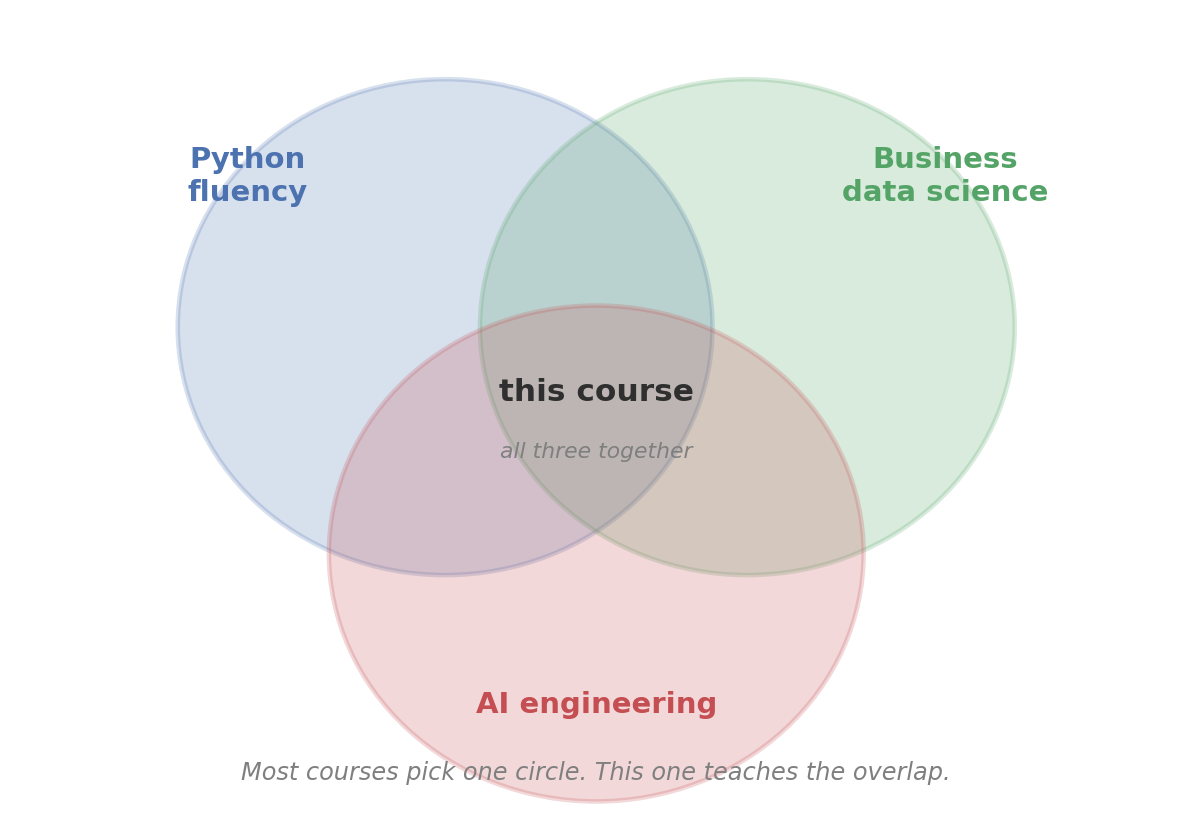
\includegraphics[width=0.9\textwidth,height=0.78\textheight,keepaspectratio]{images/06_three_circles.png}
  \end{center}
  \note{%
    \textbf{$\sim$4 min.} Point: this is not a pure programming course, not a pure statistics course, and not a prompt-engineering course --- it is the overlap.\\[2pt]
    The overlap is the employable part: plenty of people can do one circle. Doing all three is what lets you take a business problem and return a working, defensible system.\\[2pt]
    \textbf{Ask the room:} ``Which circle are you strongest in?'' Useful for you (calibrates pace) and for them (they find their pairs).
  }
\end{frame}

\begin{frame}{Three skills, taught together}
  \begin{block}{1. Python fluency}
    Read, write, and modify clean Python without friction. Functions, modules, error handling, defensive parsing.
  \end{block}
  \begin{exampleblock}{2. Working with data professionally}
    pandas, NumPy, matplotlib, scikit-learn, statistics, time-series forecasting --- plus PyTorch deep learning for when the classical toolkit stops. Real datasets, not toy ones.
  \end{exampleblock}
  \begin{block}{3. AI-driven automation}
    Calling LLMs as functions. Structured output. Retrieval-augmented generation. Tools and agents. Document processing. \emph{Plus} the engineering wrapper around all of it.
  \end{block}
  \note{%
    \textbf{$\sim$6 min.} Point: name the three skills concretely so ``AI course'' stops being vague.\\[2pt]
    \textbf{The phrase to land is ``LLMs as functions.''} Most students arrive thinking of AI as a chat window. This course treats a model as a component you call from code, with typed inputs and outputs, inside a program you control. That reframe is most of the difference between a demo and a product.\\[2pt]
    Stress ``real datasets, not toy ones'' --- they'll meet messy data early, on purpose.\\[2pt]
    ``The engineering wrapper'' is the honest bit: evaluation, cost, monitoring, deployment. It's the least glamorous and the most decisive.
  }
\end{frame}

% ============================================================
\section{Structure}
% ============================================================

\begin{frame}{Twenty modules --- 53 lessons, 7 labs (+ 14 appendices)}
  \scriptsize
  \renewcommand{\arraystretch}{0.88}%
  \begin{tabular}{rll}
    \toprule
    \textbf{\#} & \textbf{Module} & \textbf{Notebooks} \\
    \midrule
    0 & Onboarding              & master onboarding + overview + see-it-work \\
    1 & Foundations             & NB 1–6 — Python you can read without friction \\
    2 & Data science            & NB 7–11 — pandas, NumPy, plots, stats, time series \\
    3 & Real-world I/O          & NB 12–13 — HTTP, SQL, validation \\
    4 & Web scraping            & NB 14–16 — BeautifulSoup, Firecrawl, the OpenAlex API \\
    5 & Machine learning        & NB 17–19 — sklearn, model evaluation, features \\
    6 & Deep learning (PyTorch) & NB 20–22 — tensors \& the training loop, training craft, embeddings \& serving \\
    7 & Industry applications   & NB 23–26 — churn value, fraud, segmentation, demand \\
    8 & AI engineering          & NB 27–32 — LLM patterns, RAG, agents, evaluation \\
    9 & Building AI POCs        & NB 33–36 — setup, three POCs, RAG deep dive, agentic AI \\
    10 & Agents, tools \& MCP    & NB 37–40 — architectures, robust tools, MCP, multi-agent \\
    11 & NLP (optional)          & NB 41–43 — topic modeling, sentiment \\
    12 & DeepTab (optional)      & NB 44 — deep learning for tabular data \\
    13 & Production              & NB 45–46 — packaging, scheduling, config \& secrets \\
    14 & CI/CD \& deployment     & mini-book + 3 labs — Docker, GitHub Actions, HTTPS \\
    15 & Capstones               & NB 47–48 — analytics + AI assistant \\
    16 & Business AI             & NB 49–52 — strategy, architecture, BPM, governance \\
    17 & Django (optional)       & mini-book + 2 labs — serve a model behind a web UI \\
    18 & Compound AI eval (opt.) & NB 53 + lab — factorial designs, ANOVA attribution, CAFE \\
    19 & Containers (optional)   & mini-book + lab — images, layers, namespaces, Dockerfiles \\
    \bottomrule
  \end{tabular}
  \vspace{4pt}

  {\footnotesize \textbf{Every module folder has its own README} --- goals, prerequisites, what you'll build. Read it before the module's first notebook. Module and lesson numbers follow the learning order.}
  \note{%
    \textbf{$\sim$8 min.} Point: the full map. Let them \emph{scan} --- don't narrate 20 rows.\\[2pt]
    Call out only the shape: modules 1--5 are the skill spine, 7--12 the applications, 13--19 the shipping and judgement half. Then name the optional ones (11, 12, 14, 17, 18, 19) explicitly --- that's the anxiety reducer.\\[2pt]
    \textbf{The footnote is the actionable instruction:} every module has a README with goals and prerequisites. Students who skip them get lost; students who read them never wonder whether they're ready.\\[2pt]
    \textbf{Ask the room:} ``Anything here you're surprised to see in an AI course?'' Usually CI/CD or Django --- and the answer is the whole thesis: shipping is the job.\\[2pt]
    \emph{Maintainer note:} the counts on this slide and the study slide are hand-maintained. If you've added a module, re-check them against the repo README.
  }
\end{frame}

\begin{frame}{Module dependencies — what comes before what}
  \begin{center}
    
\includegraphics[width=\textwidth,height=0.82\textheight,keepaspectratio]{images/01_dependency_graph.png}
  \end{center}
  \note{%
    \textbf{$\sim$5 min.} Point: it is a graph, not a queue --- several modules are safe to take in any order once their upstreams are done.\\[2pt]
    Use it to answer the question they're all silently asking: ``can I skip ahead to the AI parts?'' Follow the edges into module 8 --- it needs 3 and 5. Skipping means you'll be debugging pandas errors instead of learning AI engineering.\\[2pt]
    Note module 19 sits as a root: it needs only Module-1 Python and a terminal, so it can be read any time --- before or after module 14.\\[2pt]
    This graph is generated from the repo's module tables, so it stays true after a renumber.
  }
\end{frame}

% ============================================================
\section{Learning paths}
% ============================================================

\begin{frame}{Pick the path that fits you}
  \begin{center}
    
\includegraphics[width=\textwidth,height=0.82\textheight,keepaspectratio]{images/02_learning_paths.png}
  \end{center}
  \note{%
    \textbf{$\sim$4 min.} Point: five paths, wildly different time budgets --- 10 h to 125 h. Nobody does all of it unless they want to.\\[2pt]
    Let them find their row and read across. The greyed dots are modules that path skips, and skipping is \emph{endorsed}, not a compromise.\\[2pt]
    For a taught cohort, say plainly which path your syllabus follows and which modules are examinable --- otherwise this slide creates uncertainty rather than removing it.\\[2pt]
    Next slide has the detail; keep this one to orientation.
  }
\end{frame}

\begin{frame}{When to pick which path}
  \begin{block}{Complete beginner}
    Never written code before. Take all modules in \textbf{spiral order} (see it work first, then the skills, then the builds). Time-budget: \textbf{about 125 hours} — the interactive estimator in \texttt{00b} computes yours.
  \end{block}
  \begin{exampleblock}{Analyst who knows Excel and SQL}
    Skim Module 1 (Python basics); Module 3's SQL will feel familiar. Focus on Modules 2 (data science), 4 (web scraping), 5 (ML), 7 (industry applications), 15 (capstone). Time-budget: \textbf{about 47 hours}.
  \end{exampleblock}
  \begin{block}{ML practitioner adding AI engineering}
    Skip foundations and data science. Focus on Modules 6 (PyTorch), 8 (AI engineering), 10 (agents \& MCP), 13 (production), 15 (capstone). Time-budget: \textbf{about 38 hours}.
  \end{block}
  \note{%
    \textbf{$\sim$8 min.} Point: give explicit permission to skip. The most common failure is a capable analyst grinding through Module 1 out of duty and quitting from boredom.\\[2pt]
    The instruction that matters: \textbf{skim, don't skip blind.} Open the module README, check the goals, and if you can already do all of them, move on --- and come back the moment something doesn't parse.\\[2pt]
    \textbf{The hour figures are honest and worth defending} --- 125 hours for a true beginner. Underselling it produces dropouts at week three. The estimator in notebook 00b computes a personal number from their answers.\\[2pt]
    \textbf{Ask the room:} ``Which of these three is closest to you?'' Hands up per path --- tells you instantly what pace the cohort needs.
  }
\end{frame}

\begin{frame}{Twelve weeks, self-paced}
  \begin{center}
    
\includegraphics[width=\textwidth,height=0.65\textheight,keepaspectratio]{images/03_weekly_timeline.png}
  \end{center}
  Got more time? Move faster. Got less? Split one week into two.
  \note{%
    \textbf{$\sim$4 min.} Point: a concrete, self-paced 12-week shape --- 8--15 h/week. This is the answer to ``how long will this actually take?''\\[2pt]
    Note the weeks are not uniform: week 11 (POCs $+$ agents) is the heaviest at $\sim$15 h. Flag it now so it isn't a surprise.\\[2pt]
    \textbf{If you're teaching this as a taught course, say clearly that this is the self-paced plan and your lecture schedule differs} --- otherwise students try to follow both. The fast track's 12-lecture plan is the taught-course version.\\[2pt]
    The line to say: consistency beats intensity. Six focused hours a week for twelve weeks beats two heroic weekends.
  }
\end{frame}

% ============================================================
\section{How to study}
% ============================================================

\begin{frame}{The five-step study loop}
  \begin{center}
    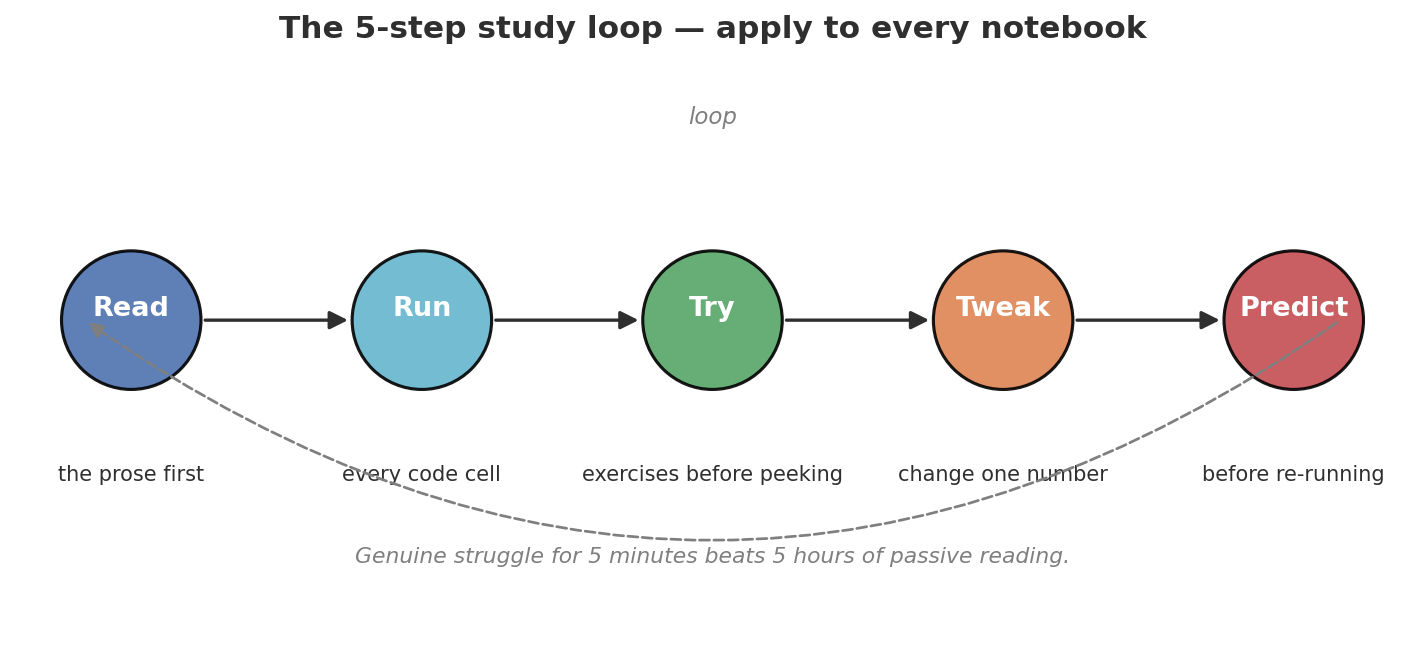
\includegraphics[width=\textwidth,height=0.65\textheight,keepaspectratio]{images/04_study_loop.png}
  \end{center}
  Apply this loop to \emph{every} notebook. Genuine struggle beats passive reading.
  \note{%
    \textbf{$\sim$6 min --- the highest-value slide for outcomes.}\\[2pt]
    Point: \emph{how} to study, not what. Read $\to$ Run $\to$ Try $\to$ Tweak $\to$ Predict.\\[2pt]
    \textbf{Predict-before-you-run is the step that does the work} and the one everyone drops. Saying the expected output out loud before pressing shift-enter converts passive reading into a test with immediate feedback. When the prediction is wrong, that's the learning moment.\\[2pt]
    Be blunt about the failure mode: running every cell and watching output scroll past feels productive and teaches almost nothing. Ask them how they'd know the difference the next morning.\\[2pt]
    \textbf{Ask the room:} ``Who has read a whole tutorial and remembered none of it?'' Every hand. That's why this slide exists.
  }
\end{frame}

\begin{frame}{Eight visual markers you'll see throughout}
  \footnotesize
  \begin{tabular}{ll}
    \toprule
    \textbf{Marker} & \textbf{Meaning} \\
    \midrule
    \texttt{(Tip)}            & A small ``stop and notice'' callout. \\
    \texttt{(Intuition)}      & The mental model behind the syntax. \\
    \texttt{(Pitfall)}        & A bug or anti-pattern that bites if you're not warned. \\
    \texttt{(Quick exercise)} & A $\sim$2-minute in-lesson checkpoint with a collapsible solution. \\
    \texttt{(Exercises)}      & Hands-on tasks. Try \emph{before} peeking at the solution. \\
    \texttt{(Bonus)}          & One larger applied task per notebook. \\
    \texttt{(Debug me)}       & A cell that \emph{intentionally} contains a bug for you to find. \\
    \texttt{(Next step)}      & Always points to the next notebook in your path. \\
    \bottomrule
  \end{tabular}
  \vspace{4pt}

  Once you internalise the markers they become road signs, not decoration.
  \note{%
    \textbf{$\sim$5 min.} Point: the notebooks have a consistent visual grammar --- learn it once, navigate 117 notebooks.\\[2pt]
    The two to dwell on: \textbf{Quick exercise} (a $\sim$2-minute checkpoint with a collapsible solution --- the rhythm of every lesson) and \textbf{Debug me} (a cell that is \emph{intentionally} broken).\\[2pt]
    \textbf{Warn them explicitly about Debug me}, or someone will spend twenty minutes assuming the course has a typo. The bug is the exercise.\\[2pt]
    Tell them to resist opening solutions early --- reading a solution feels like understanding and isn't. The struggle is where the learning is.
  }
\end{frame}

\begin{frame}{Checkpoints, quizzes, and the fast track}
  \begin{block}{322 in-lesson checkpoints --- the rhythm of every lesson}
    Roughly every $\sim$20 minutes of material: a \texttt{(Quick exercise)} with a scaffolded starter and a collapsible solution --- every solution executed in a fresh kernel. Teach $\to$ try for $\sim$2 minutes $\to$ reveal.
  \end{block}
  \begin{exampleblock}{17 module quizzes}
    Five multiple-choice questions per content module ($\sim$10 minutes) in \texttt{quizzes/} --- read code, predict behaviour, pick the right tool. Score 0--2/5? Re-do the module before moving on.
  \end{exampleblock}
  \begin{block}{Short on time? The fast track}
    \texttt{fast\_track/} condenses the whole course into 22 trimmed lessons ($\sim$26 hours) --- the 14 core essentials plus 8 breadth extensions.
  \end{block}
  \note{%
    \textbf{$\sim$6 min.} Point: three feedback mechanisms at three timescales --- checkpoints (minutes), quizzes (per module), fast track (an alternative route).\\[2pt]
    \textbf{If you're teaching live, this slide is about you as much as them:} the 322 checkpoints are the built-in pause points. Teach $\sim$20 min, set the checkpoint, give them $\sim$2 min, reveal. That's the lecture rhythm, and it needs no preparation.\\[2pt]
    The quiz rule is worth stating plainly: score 0--2 out of 5 and redo the module before moving on. The dependency graph means weak foundations compound.\\[2pt]
    Mention the fast track exists but don't oversell it to a taught cohort --- it's for people with a hard time budget, and it trims depth to get there.
  }
\end{frame}

% ============================================================
\section{What you'll build}
% ============================================================

\begin{frame}{Six small artefacts you ship along the way}
  \begin{center}
    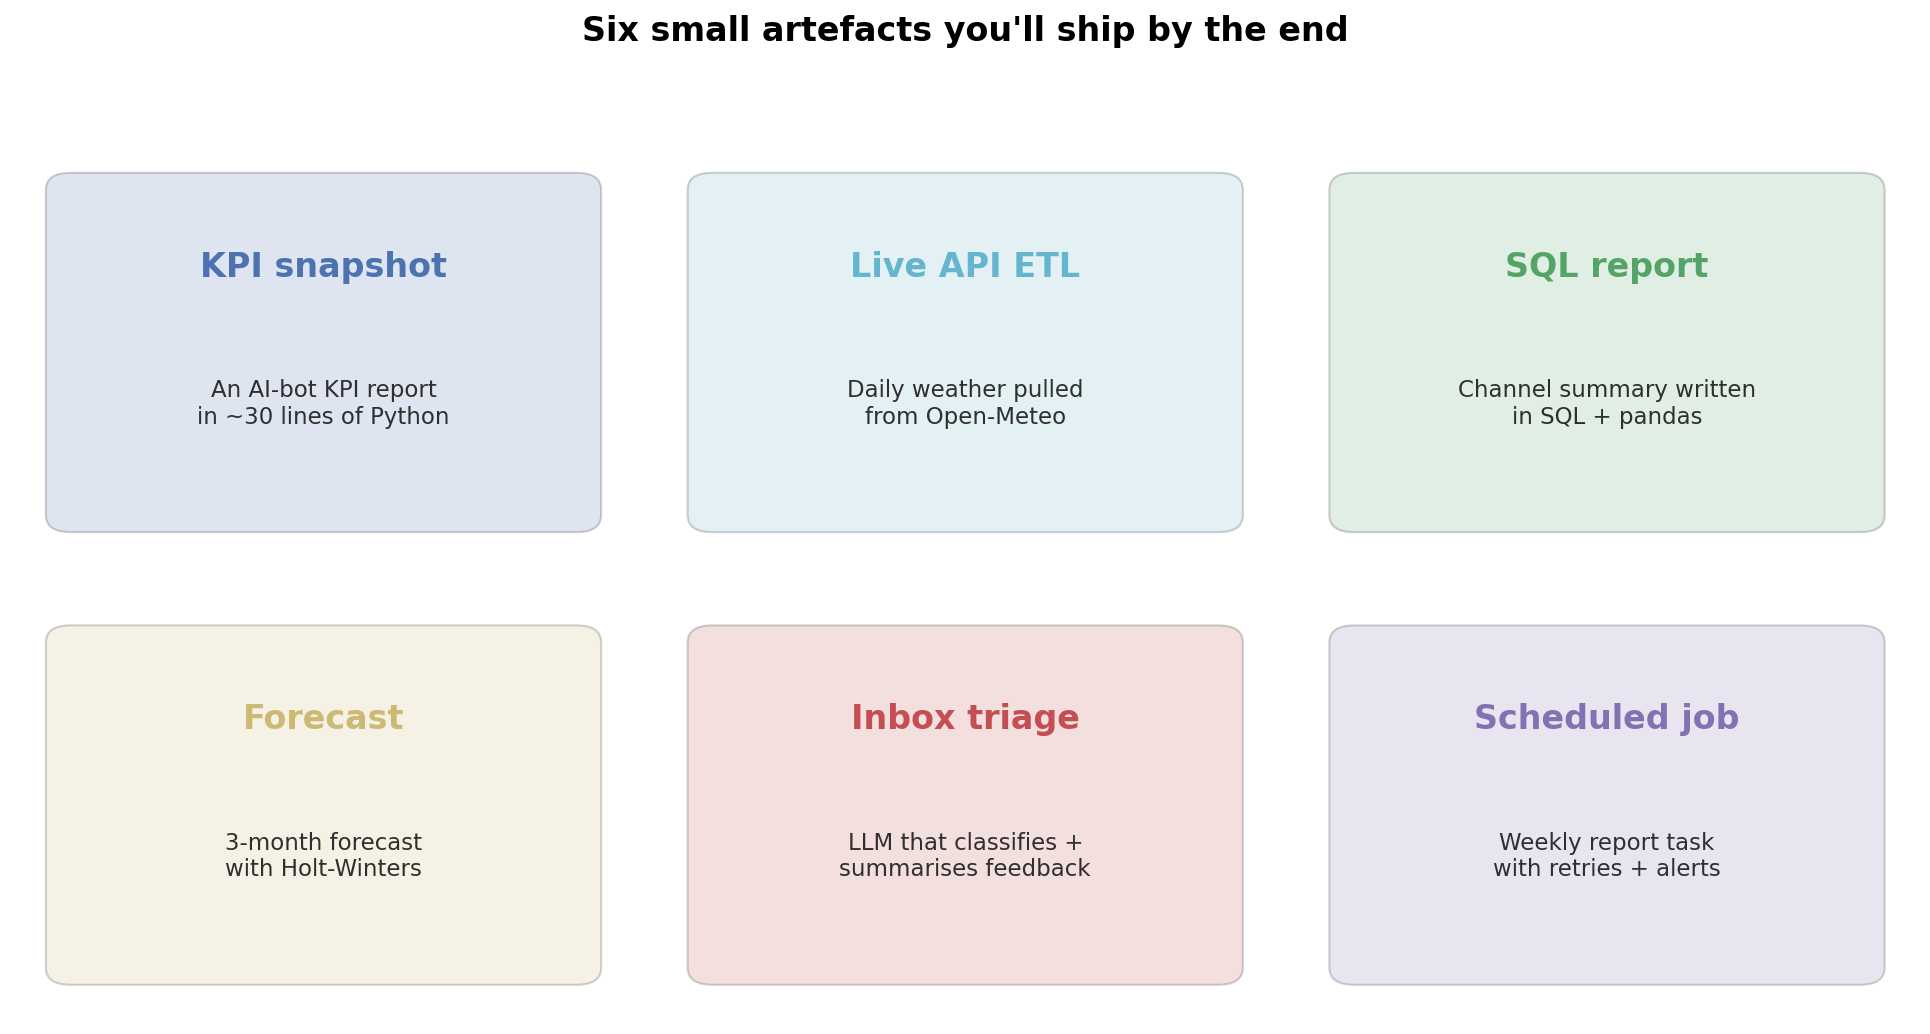
\includegraphics[width=\textwidth,height=0.82\textheight,keepaspectratio]{images/05_what_youll_build.png}
  \end{center}
  \note{%
    \textbf{$\sim$5 min.} Point: they finish with things that exist, not just notes. Motivation slide --- keep the energy up.\\[2pt]
    The framing that lands with career-minded students: these are portfolio pieces you can show and \emph{explain}. Being able to defend a design decision in an interview is what separates them from someone who followed a tutorial.\\[2pt]
    Keep it brief --- the detail is in the modules, and the capstones are on the next slide.
  }
\end{frame}

\begin{frame}{Plus two big capstones at the end}
  \begin{exampleblock}{Capstone A — AI Support-Bot Analytics (NB 47)}
    Five channels × twelve months of operational data $\to$ 2$\times$2 executive dashboard $\to$ regression demonstrating Simpson's paradox $\to$ five-bullet executive summary.
  \end{exampleblock}
  \vspace{6pt}
  \begin{block}{Capstone B — AI Customer-Feedback Assistant (NB 48)}
    Ingest free-form customer feedback $\to$ classify + extract via the MockLLM $\to$ ground answers in a knowledge base via RAG $\to$ orchestrate as a scheduled job with alerts. End-to-end AI feature.
  \end{block}
  \note{%
    \textbf{$\sim$6 min.} Point: two capstones, deliberately different --- A is the analytics story, B is the AI system.\\[2pt]
    \textbf{Capstone A's real lesson is Simpson's paradox} --- the aggregate trend reverses when you segment. It's the single most useful statistical trap for anyone presenting numbers to management, and it lands far harder in a project than on a slide.\\[2pt]
    Capstone B is the whole AI-engineering stack in one artefact: classify, extract, ground with RAG, schedule, alert. If they can explain that pipeline, they can hold a technical conversation about production AI.\\[2pt]
    Both end in a \emph{decision or a summary a manager could act on} --- that's the course's signature, and it's what makes them portfolio-worthy.
  }
\end{frame}

% ============================================================
\section{Getting started}
% ============================================================

\begin{frame}{LLM providers — local and hosted, four options}
  \footnotesize
  \begin{tabular}{lll}
    \toprule
    \textbf{Provider} & \textbf{Class} & \textbf{Best for} \\
    \midrule
    OpenAI    & \texttt{OpenAILLM("gpt-5.4-mini")}            & Reliable default \\
    Anthropic & \texttt{AnthropicLLM("claude-haiku-4-5")}    & Long context, careful tone \\
    Google    & \texttt{GoogleLLM("gemini-2.5-flash")}       & Cheapest at high volume \\
    Ollama    & \texttt{OllamaLLM("llama3.2:3b")}            & \textbf{Local} -- no internet, no key \\
    \bottomrule
  \end{tabular}
  \vspace{6pt}
  \begin{block}{Default = the offline MockLLM}
    Every AI notebook runs offline by default. Swapping in a real provider is a
    \emph{one-line} change thanks to the unified interface in
    \texttt{llm\_providers.py} at the repo root.
  \end{block}
  \vspace{4pt}
  \begin{exampleblock}{See the dedicated guide}
    Notebook \texttt{08\_ai\_engineering/A1\_llm\_providers\_guide.ipynb} has the
    full setup walk-through, model recommendations, and cost estimates.
  \end{exampleblock}
  \note{%
    \textbf{$\sim$6 min.} Point: the course is \textbf{100\,\% offline by default}. Say this early and clearly --- it removes the biggest barrier and the biggest anxiety.\\[2pt]
    \textbf{Nobody needs an API key, a credit card, or an account to complete this course.} Every AI notebook runs against a built-in MockLLM. Repeat it; students who half-heard it will worry for weeks.\\[2pt]
    Swapping in a real provider is a one-line change through the shared interface in \texttt{llm\_providers.py} --- that's a service-oriented boundary, and NB 50 names it as one.\\[2pt]
    \emph{Maintainer note:} the model names here mirror the defaults in \texttt{llm\_providers.py}. If you update one, update the other --- and expect this table to date quickly.
  }
\end{frame}


\begin{frame}[fragile]{What you need to install}
  \begin{block}{For Google Colab}
    Nothing. All required libraries are pre-installed. Open the notebook, hit Shift+Enter.
  \end{block}
  \begin{exampleblock}{For local Jupyter}
\small
\begin{verbatim}
python -m venv .venv
source .venv/bin/activate
pip install -r requirements.txt
jupyter lab
\end{verbatim}
  \end{exampleblock}
  Notebook 0 includes an environment-check cell you run to confirm everything works before you move on.
  \note{%
    \textbf{$\sim$8 min --- and budget more if this is session one with a fresh cohort.}\\[2pt]
    Point: two routes in. \textbf{Colab needs nothing} --- that is the answer for anyone whose laptop is fighting them, and it takes setup off the critical path entirely.\\[2pt]
    \textbf{If you're teaching live, do the local setup with the room now}, not later. Environment problems are the number-one reason people quietly stop, and they're much cheaper to fix with a neighbour than alone at home. Expect the usual: wrong Python version, activation not persisting, corporate proxies.\\[2pt]
    Point everyone at the environment-check cell in notebook 0 --- it's the definitive answer to ``is my setup right?''\\[2pt]
    \textbf{Have the Colab link ready as the escape hatch} for anyone still stuck after ten minutes; move on and debug in the break.
  }
\end{frame}

\begin{frame}[fragile]{Now → open Notebook 0}
  \vspace{8pt}
  \begin{center}
    {\large One file to open. The rest unfolds from there.}\\[14pt]
    \texttt{\large 00\_onboarding/00\_master\_onboarding.ipynb}\\[18pt]
  \end{center}
  \begin{block}{Three things that notebook does for you}
    \begin{enumerate}
      \item Confirms your Python environment is correctly set up.
      \item Explains the five-step study loop you'll use throughout.
      \item Helps you pick the right learning path from the five options.
    \end{enumerate}
  \end{block}
  \note{%
    \textbf{$\sim$4 min.} Point: reduce the whole deck to one action --- open one file.\\[2pt]
    The most common way to fail at this course is never starting because 117 notebooks feels like too much. One file. The rest unfolds.\\[2pt]
    \textbf{If you have five minutes, open it on screen now} and let them watch the environment check run. Seeing it work is worth more than describing it.\\[2pt]
    If your cohort is following a fixed syllabus, say so here so nobody spends an evening on the path-picker.
  }
\end{frame}

\begin{frame}{One last reminder before you start}
  \begin{block}{Five-step study loop, in your pocket}
    \textbf{Read} the prose first $\to$ \textbf{Run} every code cell $\to$
    \textbf{Try} the exercises before peeking $\to$ \textbf{Tweak} one number $\to$
    \textbf{Predict} the new output before re-running.
  \end{block}
  \begin{exampleblock}{When to use which marker}
    \texttt{(Tip)} information; \texttt{(Intuition)} mental model;
    \texttt{(Pitfall)} avoid this; \texttt{(Quick exercise)} $\sim$2-minute checkpoint;
    \texttt{(Exercise)} hands-on practice; \texttt{(Bonus)} bigger applied task;
    \texttt{(Debug me)} intentional bug — find it.
  \end{exampleblock}
  \begin{alertblock}{When you're stuck for 15 minutes}
    Copy the full error into a search engine. 95\% of beginner errors are
    well-documented. The course is designed to teach you to debug, not to
    spare you the experience.
  \end{alertblock}
  \note{%
    \textbf{$\sim$5 min.} Point: the debugging attitude. This is the slide that keeps people from quitting in week two.\\[2pt]
    \textbf{Normalise the errors:} a red traceback is not a sign they're unsuited to this. Professionals see them all day; the difference is they read them instead of panicking. Tell them to read the \emph{last} line first.\\[2pt]
    The 15-minute rule is a real technique --- struggle is productive up to a point, then it's just attrition. Search the exact error text, then ask a person.\\[2pt]
    Nice callback: NB 27 explains \emph{why} the assistant will confidently invent a fix; NB 51 gives the review checklist. The course teaches supervision, not avoidance.\\[2pt]
    If you're teaching live, this is where you name your office hours or forum. Say it concretely.
  }
\end{frame}

\begin{frame}
  \begin{center}
    {\Huge\bfseries Welcome.}\\[10pt]
    \large 117 notebooks await you.\\[20pt]
    {\large \textit{Open Module 0 next.}}
  \end{center}
  \note{%
    \textbf{$\sim$2 min --- close warmly and stop.}\\[2pt]
    Point: end on the invitation, not on logistics. Resist adding one more announcement here.\\[2pt]
    If you want one closing line, make it the promise the course actually keeps: \emph{by the end, you will have shipped something that runs, and you'll be able to explain every part of it.}\\[2pt]
    Then give the single next action out loud --- open \texttt{00\_master\_onboarding.ipynb} before the next session --- and take questions.
  }
\end{frame}

\end{document}
"
\ifdefined\notesmode
  \usepackage{pgfpages}
  \setbeameroption{show notes on second screen=right}
\fi

% Theme
\usetheme{Madrid}
\usecolortheme{default}
\setbeamertemplate{navigation symbols}{}
\setbeamertemplate{footline}[frame number]
\setbeamertemplate{blocks}[rounded][shadow=false]
\setbeamertemplate{headline}{%
  \leavevmode%
  \hbox{%
    \begin{beamercolorbox}[wd=\paperwidth,ht=2.5ex,dp=1.125ex]{section in head/foot}%
      \insertsectionnavigationhorizontal{\paperwidth}{}{\hskip0pt plus1filll}%
    \end{beamercolorbox}%
  }%
}
\AtBeginSection[]{%
  \begin{frame}{Outline}
    \tableofcontents[currentsection,sectionstyle=show/shaded,subsectionstyle=show/show/hide]
  \end{frame}
}

\title{Course Overview}
\subtitle{Python for AI-Driven Automation and Business Data Science}
\author{Course materials}
\institute{}
\date{}

\begin{document}

\begin{frame}\titlepage\end{frame}

\begin{frame}{Contents}
  \tableofcontents[hideallsubsections]
\end{frame}

% ============================================================
\section{The big picture}
% ============================================================

\begin{frame}{The course in one diagram}
  \begin{center}
    
\includegraphics[width=\textwidth,height=0.78\textheight,keepaspectratio]{images/00_course_roadmap.png}
  \end{center}
  \note{%
    \textbf{$\sim$5 min.} Point: show the whole shape once, so everything later has somewhere to attach.\\[2pt]
    Trace the spine with a finger --- Python $\to$ data $\to$ ML $\to$ AI $\to$ shipping --- and say the one sentence that matters: \textbf{each module is a prerequisite for the next, so the order is not arbitrary.}\\[2pt]
    Point out the starred optional modules now to defuse the intimidation: 20 modules is not 20 obligations.\\[2pt]
    \textbf{Do not read the boxes aloud.} They will read faster than you can speak, and the detail comes three slides later.
  }
\end{frame}

\begin{frame}{Where this course sits}
  \begin{center}
    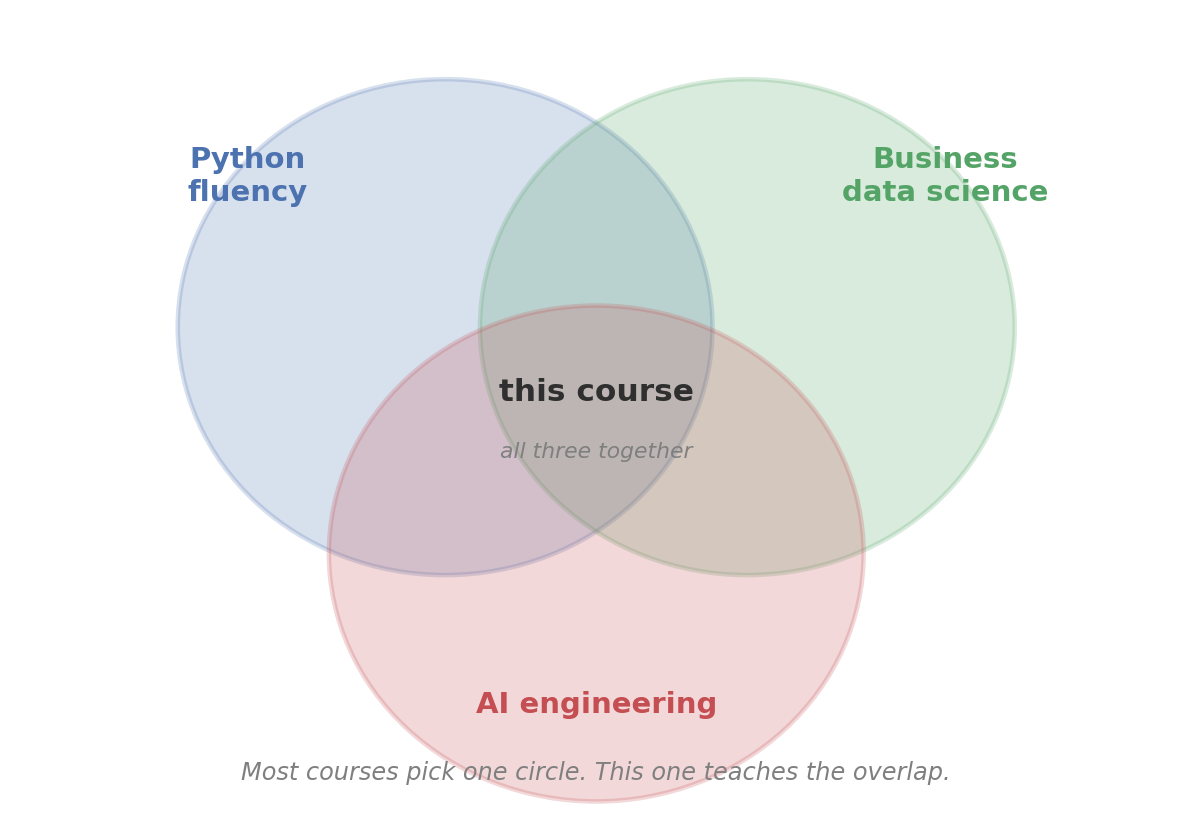
\includegraphics[width=0.9\textwidth,height=0.78\textheight,keepaspectratio]{images/06_three_circles.png}
  \end{center}
  \note{%
    \textbf{$\sim$4 min.} Point: this is not a pure programming course, not a pure statistics course, and not a prompt-engineering course --- it is the overlap.\\[2pt]
    The overlap is the employable part: plenty of people can do one circle. Doing all three is what lets you take a business problem and return a working, defensible system.\\[2pt]
    \textbf{Ask the room:} ``Which circle are you strongest in?'' Useful for you (calibrates pace) and for them (they find their pairs).
  }
\end{frame}

\begin{frame}{Three skills, taught together}
  \begin{block}{1. Python fluency}
    Read, write, and modify clean Python without friction. Functions, modules, error handling, defensive parsing.
  \end{block}
  \begin{exampleblock}{2. Working with data professionally}
    pandas, NumPy, matplotlib, scikit-learn, statistics, time-series forecasting --- plus PyTorch deep learning for when the classical toolkit stops. Real datasets, not toy ones.
  \end{exampleblock}
  \begin{block}{3. AI-driven automation}
    Calling LLMs as functions. Structured output. Retrieval-augmented generation. Tools and agents. Document processing. \emph{Plus} the engineering wrapper around all of it.
  \end{block}
  \note{%
    \textbf{$\sim$6 min.} Point: name the three skills concretely so ``AI course'' stops being vague.\\[2pt]
    \textbf{The phrase to land is ``LLMs as functions.''} Most students arrive thinking of AI as a chat window. This course treats a model as a component you call from code, with typed inputs and outputs, inside a program you control. That reframe is most of the difference between a demo and a product.\\[2pt]
    Stress ``real datasets, not toy ones'' --- they'll meet messy data early, on purpose.\\[2pt]
    ``The engineering wrapper'' is the honest bit: evaluation, cost, monitoring, deployment. It's the least glamorous and the most decisive.
  }
\end{frame}

% ============================================================
\section{Structure}
% ============================================================

\begin{frame}{Twenty modules --- 53 lessons, 7 labs (+ 14 appendices)}
  \scriptsize
  \renewcommand{\arraystretch}{0.88}%
  \begin{tabular}{rll}
    \toprule
    \textbf{\#} & \textbf{Module} & \textbf{Notebooks} \\
    \midrule
    0 & Onboarding              & master onboarding + overview + see-it-work \\
    1 & Foundations             & NB 1–6 — Python you can read without friction \\
    2 & Data science            & NB 7–11 — pandas, NumPy, plots, stats, time series \\
    3 & Real-world I/O          & NB 12–13 — HTTP, SQL, validation \\
    4 & Web scraping            & NB 14–16 — BeautifulSoup, Firecrawl, the OpenAlex API \\
    5 & Machine learning        & NB 17–19 — sklearn, model evaluation, features \\
    6 & Deep learning (PyTorch) & NB 20–22 — tensors \& the training loop, training craft, embeddings \& serving \\
    7 & Industry applications   & NB 23–26 — churn value, fraud, segmentation, demand \\
    8 & AI engineering          & NB 27–32 — LLM patterns, RAG, agents, evaluation \\
    9 & Building AI POCs        & NB 33–36 — setup, three POCs, RAG deep dive, agentic AI \\
    10 & Agents, tools \& MCP    & NB 37–40 — architectures, robust tools, MCP, multi-agent \\
    11 & NLP (optional)          & NB 41–43 — topic modeling, sentiment \\
    12 & DeepTab (optional)      & NB 44 — deep learning for tabular data \\
    13 & Production              & NB 45–46 — packaging, scheduling, config \& secrets \\
    14 & CI/CD \& deployment     & mini-book + 3 labs — Docker, GitHub Actions, HTTPS \\
    15 & Capstones               & NB 47–48 — analytics + AI assistant \\
    16 & Business AI             & NB 49–52 — strategy, architecture, BPM, governance \\
    17 & Django (optional)       & mini-book + 2 labs — serve a model behind a web UI \\
    18 & Compound AI eval (opt.) & NB 53 + lab — factorial designs, ANOVA attribution, CAFE \\
    19 & Containers (optional)   & mini-book + lab — images, layers, namespaces, Dockerfiles \\
    \bottomrule
  \end{tabular}
  \vspace{4pt}

  {\footnotesize \textbf{Every module folder has its own README} --- goals, prerequisites, what you'll build. Read it before the module's first notebook. Module and lesson numbers follow the learning order.}
  \note{%
    \textbf{$\sim$8 min.} Point: the full map. Let them \emph{scan} --- don't narrate 20 rows.\\[2pt]
    Call out only the shape: modules 1--5 are the skill spine, 7--12 the applications, 13--19 the shipping and judgement half. Then name the optional ones (11, 12, 14, 17, 18, 19) explicitly --- that's the anxiety reducer.\\[2pt]
    \textbf{The footnote is the actionable instruction:} every module has a README with goals and prerequisites. Students who skip them get lost; students who read them never wonder whether they're ready.\\[2pt]
    \textbf{Ask the room:} ``Anything here you're surprised to see in an AI course?'' Usually CI/CD or Django --- and the answer is the whole thesis: shipping is the job.\\[2pt]
    \emph{Maintainer note:} the counts on this slide and the study slide are hand-maintained. If you've added a module, re-check them against the repo README.
  }
\end{frame}

\begin{frame}{Module dependencies — what comes before what}
  \begin{center}
    
\includegraphics[width=\textwidth,height=0.82\textheight,keepaspectratio]{images/01_dependency_graph.png}
  \end{center}
  \note{%
    \textbf{$\sim$5 min.} Point: it is a graph, not a queue --- several modules are safe to take in any order once their upstreams are done.\\[2pt]
    Use it to answer the question they're all silently asking: ``can I skip ahead to the AI parts?'' Follow the edges into module 8 --- it needs 3 and 5. Skipping means you'll be debugging pandas errors instead of learning AI engineering.\\[2pt]
    Note module 19 sits as a root: it needs only Module-1 Python and a terminal, so it can be read any time --- before or after module 14.\\[2pt]
    This graph is generated from the repo's module tables, so it stays true after a renumber.
  }
\end{frame}

% ============================================================
\section{Learning paths}
% ============================================================

\begin{frame}{Pick the path that fits you}
  \begin{center}
    
\includegraphics[width=\textwidth,height=0.82\textheight,keepaspectratio]{images/02_learning_paths.png}
  \end{center}
  \note{%
    \textbf{$\sim$4 min.} Point: five paths, wildly different time budgets --- 10 h to 125 h. Nobody does all of it unless they want to.\\[2pt]
    Let them find their row and read across. The greyed dots are modules that path skips, and skipping is \emph{endorsed}, not a compromise.\\[2pt]
    For a taught cohort, say plainly which path your syllabus follows and which modules are examinable --- otherwise this slide creates uncertainty rather than removing it.\\[2pt]
    Next slide has the detail; keep this one to orientation.
  }
\end{frame}

\begin{frame}{When to pick which path}
  \begin{block}{Complete beginner}
    Never written code before. Take all modules in \textbf{spiral order} (see it work first, then the skills, then the builds). Time-budget: \textbf{about 125 hours} — the interactive estimator in \texttt{00b} computes yours.
  \end{block}
  \begin{exampleblock}{Analyst who knows Excel and SQL}
    Skim Module 1 (Python basics); Module 3's SQL will feel familiar. Focus on Modules 2 (data science), 4 (web scraping), 5 (ML), 7 (industry applications), 15 (capstone). Time-budget: \textbf{about 47 hours}.
  \end{exampleblock}
  \begin{block}{ML practitioner adding AI engineering}
    Skip foundations and data science. Focus on Modules 6 (PyTorch), 8 (AI engineering), 10 (agents \& MCP), 13 (production), 15 (capstone). Time-budget: \textbf{about 38 hours}.
  \end{block}
  \note{%
    \textbf{$\sim$8 min.} Point: give explicit permission to skip. The most common failure is a capable analyst grinding through Module 1 out of duty and quitting from boredom.\\[2pt]
    The instruction that matters: \textbf{skim, don't skip blind.} Open the module README, check the goals, and if you can already do all of them, move on --- and come back the moment something doesn't parse.\\[2pt]
    \textbf{The hour figures are honest and worth defending} --- 125 hours for a true beginner. Underselling it produces dropouts at week three. The estimator in notebook 00b computes a personal number from their answers.\\[2pt]
    \textbf{Ask the room:} ``Which of these three is closest to you?'' Hands up per path --- tells you instantly what pace the cohort needs.
  }
\end{frame}

\begin{frame}{Twelve weeks, self-paced}
  \begin{center}
    
\includegraphics[width=\textwidth,height=0.65\textheight,keepaspectratio]{images/03_weekly_timeline.png}
  \end{center}
  Got more time? Move faster. Got less? Split one week into two.
  \note{%
    \textbf{$\sim$4 min.} Point: a concrete, self-paced 12-week shape --- 8--15 h/week. This is the answer to ``how long will this actually take?''\\[2pt]
    Note the weeks are not uniform: week 11 (POCs $+$ agents) is the heaviest at $\sim$15 h. Flag it now so it isn't a surprise.\\[2pt]
    \textbf{If you're teaching this as a taught course, say clearly that this is the self-paced plan and your lecture schedule differs} --- otherwise students try to follow both. The fast track's 12-lecture plan is the taught-course version.\\[2pt]
    The line to say: consistency beats intensity. Six focused hours a week for twelve weeks beats two heroic weekends.
  }
\end{frame}

% ============================================================
\section{How to study}
% ============================================================

\begin{frame}{The five-step study loop}
  \begin{center}
    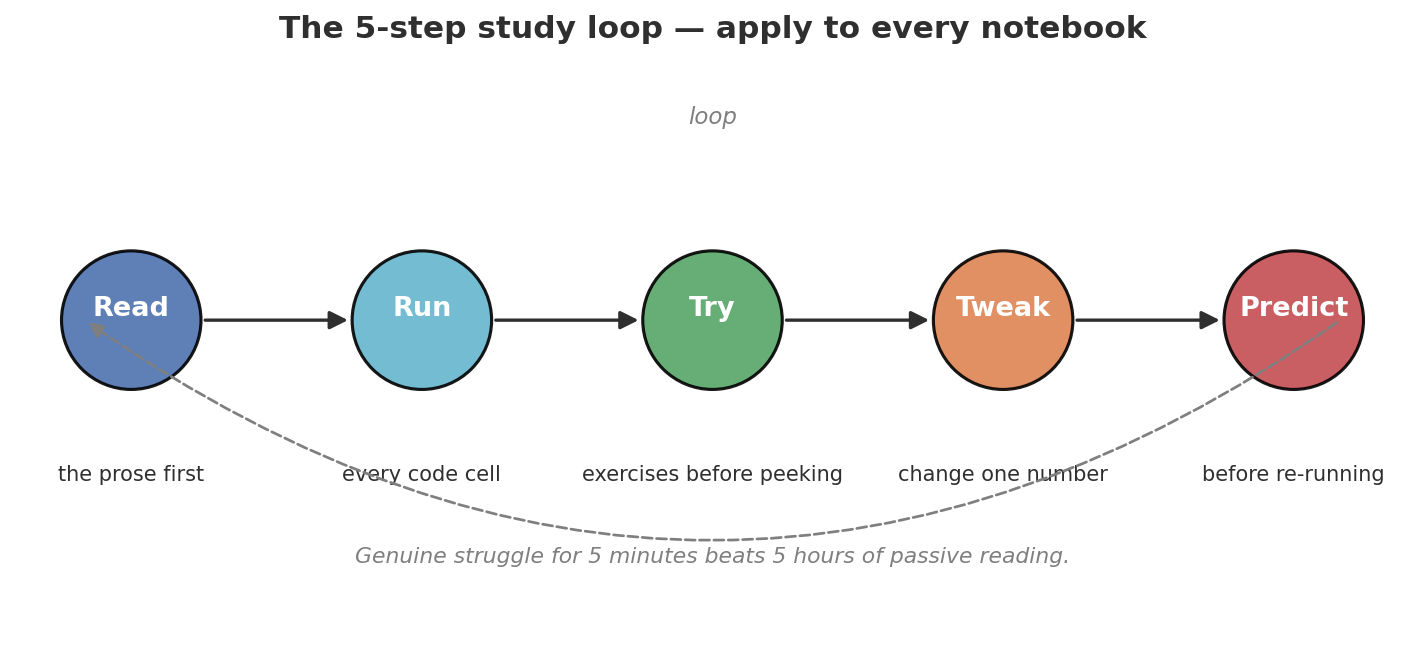
\includegraphics[width=\textwidth,height=0.65\textheight,keepaspectratio]{images/04_study_loop.png}
  \end{center}
  Apply this loop to \emph{every} notebook. Genuine struggle beats passive reading.
  \note{%
    \textbf{$\sim$6 min --- the highest-value slide for outcomes.}\\[2pt]
    Point: \emph{how} to study, not what. Read $\to$ Run $\to$ Try $\to$ Tweak $\to$ Predict.\\[2pt]
    \textbf{Predict-before-you-run is the step that does the work} and the one everyone drops. Saying the expected output out loud before pressing shift-enter converts passive reading into a test with immediate feedback. When the prediction is wrong, that's the learning moment.\\[2pt]
    Be blunt about the failure mode: running every cell and watching output scroll past feels productive and teaches almost nothing. Ask them how they'd know the difference the next morning.\\[2pt]
    \textbf{Ask the room:} ``Who has read a whole tutorial and remembered none of it?'' Every hand. That's why this slide exists.
  }
\end{frame}

\begin{frame}{Eight visual markers you'll see throughout}
  \footnotesize
  \begin{tabular}{ll}
    \toprule
    \textbf{Marker} & \textbf{Meaning} \\
    \midrule
    \texttt{(Tip)}            & A small ``stop and notice'' callout. \\
    \texttt{(Intuition)}      & The mental model behind the syntax. \\
    \texttt{(Pitfall)}        & A bug or anti-pattern that bites if you're not warned. \\
    \texttt{(Quick exercise)} & A $\sim$2-minute in-lesson checkpoint with a collapsible solution. \\
    \texttt{(Exercises)}      & Hands-on tasks. Try \emph{before} peeking at the solution. \\
    \texttt{(Bonus)}          & One larger applied task per notebook. \\
    \texttt{(Debug me)}       & A cell that \emph{intentionally} contains a bug for you to find. \\
    \texttt{(Next step)}      & Always points to the next notebook in your path. \\
    \bottomrule
  \end{tabular}
  \vspace{4pt}

  Once you internalise the markers they become road signs, not decoration.
  \note{%
    \textbf{$\sim$5 min.} Point: the notebooks have a consistent visual grammar --- learn it once, navigate 117 notebooks.\\[2pt]
    The two to dwell on: \textbf{Quick exercise} (a $\sim$2-minute checkpoint with a collapsible solution --- the rhythm of every lesson) and \textbf{Debug me} (a cell that is \emph{intentionally} broken).\\[2pt]
    \textbf{Warn them explicitly about Debug me}, or someone will spend twenty minutes assuming the course has a typo. The bug is the exercise.\\[2pt]
    Tell them to resist opening solutions early --- reading a solution feels like understanding and isn't. The struggle is where the learning is.
  }
\end{frame}

\begin{frame}{Checkpoints, quizzes, and the fast track}
  \begin{block}{322 in-lesson checkpoints --- the rhythm of every lesson}
    Roughly every $\sim$20 minutes of material: a \texttt{(Quick exercise)} with a scaffolded starter and a collapsible solution --- every solution executed in a fresh kernel. Teach $\to$ try for $\sim$2 minutes $\to$ reveal.
  \end{block}
  \begin{exampleblock}{17 module quizzes}
    Five multiple-choice questions per content module ($\sim$10 minutes) in \texttt{quizzes/} --- read code, predict behaviour, pick the right tool. Score 0--2/5? Re-do the module before moving on.
  \end{exampleblock}
  \begin{block}{Short on time? The fast track}
    \texttt{fast\_track/} condenses the whole course into 22 trimmed lessons ($\sim$26 hours) --- the 14 core essentials plus 8 breadth extensions.
  \end{block}
  \note{%
    \textbf{$\sim$6 min.} Point: three feedback mechanisms at three timescales --- checkpoints (minutes), quizzes (per module), fast track (an alternative route).\\[2pt]
    \textbf{If you're teaching live, this slide is about you as much as them:} the 322 checkpoints are the built-in pause points. Teach $\sim$20 min, set the checkpoint, give them $\sim$2 min, reveal. That's the lecture rhythm, and it needs no preparation.\\[2pt]
    The quiz rule is worth stating plainly: score 0--2 out of 5 and redo the module before moving on. The dependency graph means weak foundations compound.\\[2pt]
    Mention the fast track exists but don't oversell it to a taught cohort --- it's for people with a hard time budget, and it trims depth to get there.
  }
\end{frame}

% ============================================================
\section{What you'll build}
% ============================================================

\begin{frame}{Six small artefacts you ship along the way}
  \begin{center}
    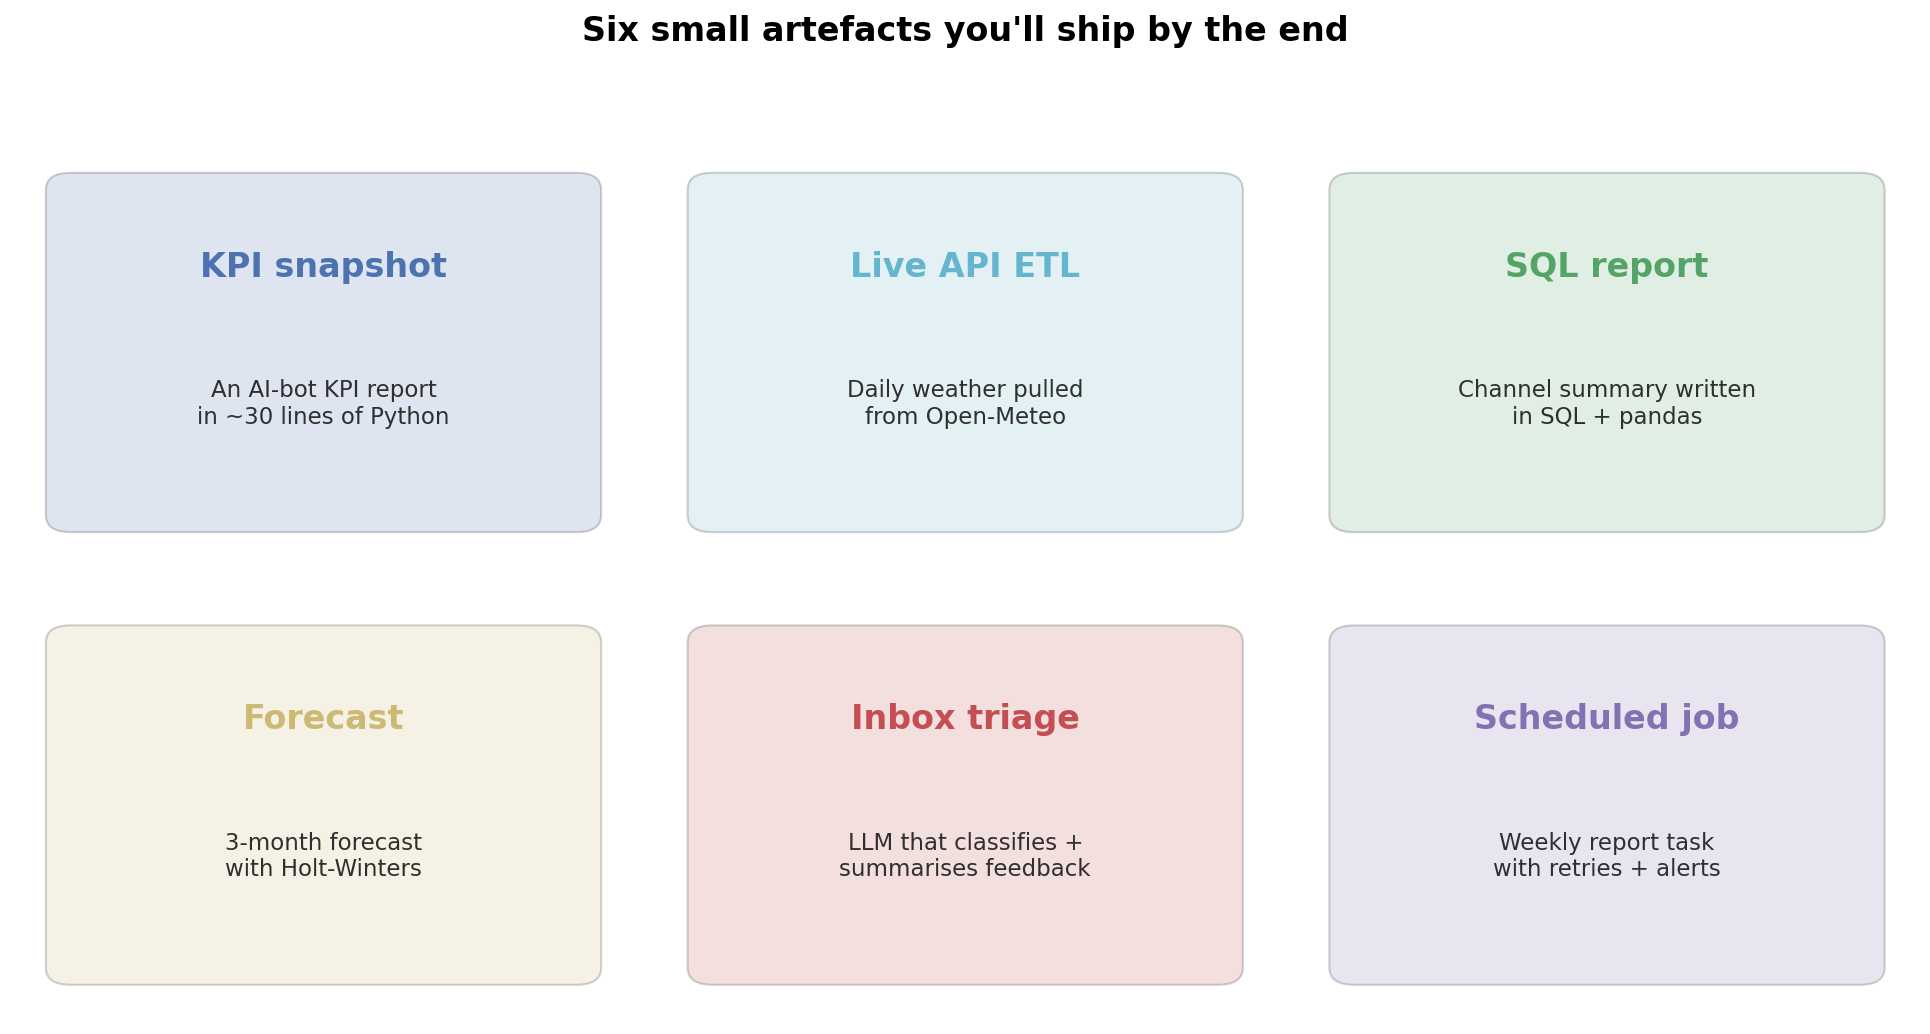
\includegraphics[width=\textwidth,height=0.82\textheight,keepaspectratio]{images/05_what_youll_build.png}
  \end{center}
  \note{%
    \textbf{$\sim$5 min.} Point: they finish with things that exist, not just notes. Motivation slide --- keep the energy up.\\[2pt]
    The framing that lands with career-minded students: these are portfolio pieces you can show and \emph{explain}. Being able to defend a design decision in an interview is what separates them from someone who followed a tutorial.\\[2pt]
    Keep it brief --- the detail is in the modules, and the capstones are on the next slide.
  }
\end{frame}

\begin{frame}{Plus two big capstones at the end}
  \begin{exampleblock}{Capstone A — AI Support-Bot Analytics (NB 47)}
    Five channels × twelve months of operational data $\to$ 2$\times$2 executive dashboard $\to$ regression demonstrating Simpson's paradox $\to$ five-bullet executive summary.
  \end{exampleblock}
  \vspace{6pt}
  \begin{block}{Capstone B — AI Customer-Feedback Assistant (NB 48)}
    Ingest free-form customer feedback $\to$ classify + extract via the MockLLM $\to$ ground answers in a knowledge base via RAG $\to$ orchestrate as a scheduled job with alerts. End-to-end AI feature.
  \end{block}
  \note{%
    \textbf{$\sim$6 min.} Point: two capstones, deliberately different --- A is the analytics story, B is the AI system.\\[2pt]
    \textbf{Capstone A's real lesson is Simpson's paradox} --- the aggregate trend reverses when you segment. It's the single most useful statistical trap for anyone presenting numbers to management, and it lands far harder in a project than on a slide.\\[2pt]
    Capstone B is the whole AI-engineering stack in one artefact: classify, extract, ground with RAG, schedule, alert. If they can explain that pipeline, they can hold a technical conversation about production AI.\\[2pt]
    Both end in a \emph{decision or a summary a manager could act on} --- that's the course's signature, and it's what makes them portfolio-worthy.
  }
\end{frame}

% ============================================================
\section{Getting started}
% ============================================================

\begin{frame}{LLM providers — local and hosted, four options}
  \footnotesize
  \begin{tabular}{lll}
    \toprule
    \textbf{Provider} & \textbf{Class} & \textbf{Best for} \\
    \midrule
    OpenAI    & \texttt{OpenAILLM("gpt-5.4-mini")}            & Reliable default \\
    Anthropic & \texttt{AnthropicLLM("claude-haiku-4-5")}    & Long context, careful tone \\
    Google    & \texttt{GoogleLLM("gemini-2.5-flash")}       & Cheapest at high volume \\
    Ollama    & \texttt{OllamaLLM("llama3.2:3b")}            & \textbf{Local} -- no internet, no key \\
    \bottomrule
  \end{tabular}
  \vspace{6pt}
  \begin{block}{Default = the offline MockLLM}
    Every AI notebook runs offline by default. Swapping in a real provider is a
    \emph{one-line} change thanks to the unified interface in
    \texttt{llm\_providers.py} at the repo root.
  \end{block}
  \vspace{4pt}
  \begin{exampleblock}{See the dedicated guide}
    Notebook \texttt{08\_ai\_engineering/A1\_llm\_providers\_guide.ipynb} has the
    full setup walk-through, model recommendations, and cost estimates.
  \end{exampleblock}
  \note{%
    \textbf{$\sim$6 min.} Point: the course is \textbf{100\,\% offline by default}. Say this early and clearly --- it removes the biggest barrier and the biggest anxiety.\\[2pt]
    \textbf{Nobody needs an API key, a credit card, or an account to complete this course.} Every AI notebook runs against a built-in MockLLM. Repeat it; students who half-heard it will worry for weeks.\\[2pt]
    Swapping in a real provider is a one-line change through the shared interface in \texttt{llm\_providers.py} --- that's a service-oriented boundary, and NB 50 names it as one.\\[2pt]
    \emph{Maintainer note:} the model names here mirror the defaults in \texttt{llm\_providers.py}. If you update one, update the other --- and expect this table to date quickly.
  }
\end{frame}


\begin{frame}[fragile]{What you need to install}
  \begin{block}{For Google Colab}
    Nothing. All required libraries are pre-installed. Open the notebook, hit Shift+Enter.
  \end{block}
  \begin{exampleblock}{For local Jupyter}
\small
\begin{verbatim}
python -m venv .venv
source .venv/bin/activate
pip install -r requirements.txt
jupyter lab
\end{verbatim}
  \end{exampleblock}
  Notebook 0 includes an environment-check cell you run to confirm everything works before you move on.
  \note{%
    \textbf{$\sim$8 min --- and budget more if this is session one with a fresh cohort.}\\[2pt]
    Point: two routes in. \textbf{Colab needs nothing} --- that is the answer for anyone whose laptop is fighting them, and it takes setup off the critical path entirely.\\[2pt]
    \textbf{If you're teaching live, do the local setup with the room now}, not later. Environment problems are the number-one reason people quietly stop, and they're much cheaper to fix with a neighbour than alone at home. Expect the usual: wrong Python version, activation not persisting, corporate proxies.\\[2pt]
    Point everyone at the environment-check cell in notebook 0 --- it's the definitive answer to ``is my setup right?''\\[2pt]
    \textbf{Have the Colab link ready as the escape hatch} for anyone still stuck after ten minutes; move on and debug in the break.
  }
\end{frame}

\begin{frame}[fragile]{Now → open Notebook 0}
  \vspace{8pt}
  \begin{center}
    {\large One file to open. The rest unfolds from there.}\\[14pt]
    \texttt{\large 00\_onboarding/00\_master\_onboarding.ipynb}\\[18pt]
  \end{center}
  \begin{block}{Three things that notebook does for you}
    \begin{enumerate}
      \item Confirms your Python environment is correctly set up.
      \item Explains the five-step study loop you'll use throughout.
      \item Helps you pick the right learning path from the five options.
    \end{enumerate}
  \end{block}
  \note{%
    \textbf{$\sim$4 min.} Point: reduce the whole deck to one action --- open one file.\\[2pt]
    The most common way to fail at this course is never starting because 117 notebooks feels like too much. One file. The rest unfolds.\\[2pt]
    \textbf{If you have five minutes, open it on screen now} and let them watch the environment check run. Seeing it work is worth more than describing it.\\[2pt]
    If your cohort is following a fixed syllabus, say so here so nobody spends an evening on the path-picker.
  }
\end{frame}

\begin{frame}{One last reminder before you start}
  \begin{block}{Five-step study loop, in your pocket}
    \textbf{Read} the prose first $\to$ \textbf{Run} every code cell $\to$
    \textbf{Try} the exercises before peeking $\to$ \textbf{Tweak} one number $\to$
    \textbf{Predict} the new output before re-running.
  \end{block}
  \begin{exampleblock}{When to use which marker}
    \texttt{(Tip)} information; \texttt{(Intuition)} mental model;
    \texttt{(Pitfall)} avoid this; \texttt{(Quick exercise)} $\sim$2-minute checkpoint;
    \texttt{(Exercise)} hands-on practice; \texttt{(Bonus)} bigger applied task;
    \texttt{(Debug me)} intentional bug — find it.
  \end{exampleblock}
  \begin{alertblock}{When you're stuck for 15 minutes}
    Copy the full error into a search engine. 95\% of beginner errors are
    well-documented. The course is designed to teach you to debug, not to
    spare you the experience.
  \end{alertblock}
  \note{%
    \textbf{$\sim$5 min.} Point: the debugging attitude. This is the slide that keeps people from quitting in week two.\\[2pt]
    \textbf{Normalise the errors:} a red traceback is not a sign they're unsuited to this. Professionals see them all day; the difference is they read them instead of panicking. Tell them to read the \emph{last} line first.\\[2pt]
    The 15-minute rule is a real technique --- struggle is productive up to a point, then it's just attrition. Search the exact error text, then ask a person.\\[2pt]
    Nice callback: NB 27 explains \emph{why} the assistant will confidently invent a fix; NB 51 gives the review checklist. The course teaches supervision, not avoidance.\\[2pt]
    If you're teaching live, this is where you name your office hours or forum. Say it concretely.
  }
\end{frame}

\begin{frame}
  \begin{center}
    {\Huge\bfseries Welcome.}\\[10pt]
    \large 117 notebooks await you.\\[20pt]
    {\large \textit{Open Module 0 next.}}
  \end{center}
  \note{%
    \textbf{$\sim$2 min --- close warmly and stop.}\\[2pt]
    Point: end on the invitation, not on logistics. Resist adding one more announcement here.\\[2pt]
    If you want one closing line, make it the promise the course actually keeps: \emph{by the end, you will have shipped something that runs, and you'll be able to explain every part of it.}\\[2pt]
    Then give the single next action out loud --- open \texttt{00\_master\_onboarding.ipynb} before the next session --- and take questions.
  }
\end{frame}

\end{document}
"
\ifdefined\notesmode
  \usepackage{pgfpages}
  \setbeameroption{show notes on second screen=right}
\fi

% Theme
\usetheme{Madrid}
\usecolortheme{default}
\setbeamertemplate{navigation symbols}{}
\setbeamertemplate{footline}[frame number]
\setbeamertemplate{blocks}[rounded][shadow=false]
\setbeamertemplate{headline}{%
  \leavevmode%
  \hbox{%
    \begin{beamercolorbox}[wd=\paperwidth,ht=2.5ex,dp=1.125ex]{section in head/foot}%
      \insertsectionnavigationhorizontal{\paperwidth}{}{\hskip0pt plus1filll}%
    \end{beamercolorbox}%
  }%
}
\AtBeginSection[]{%
  \begin{frame}{Outline}
    \tableofcontents[currentsection,sectionstyle=show/shaded,subsectionstyle=show/show/hide]
  \end{frame}
}

\title{Course Overview}
\subtitle{Python for AI-Driven Automation and Business Data Science}
\author{Course materials}
\institute{}
\date{}

\begin{document}

\begin{frame}\titlepage\end{frame}

\begin{frame}{Contents}
  \tableofcontents[hideallsubsections]
\end{frame}

% ============================================================
\section{The big picture}
% ============================================================

\begin{frame}{The course in one diagram}
  \begin{center}
    
\includegraphics[width=\textwidth,height=0.78\textheight,keepaspectratio]{images/00_course_roadmap.png}
  \end{center}
  \note{%
    \textbf{$\sim$5 min.} Point: show the whole shape once, so everything later has somewhere to attach.\\[2pt]
    Trace the spine with a finger --- Python $\to$ data $\to$ ML $\to$ AI $\to$ shipping --- and say the one sentence that matters: \textbf{each module is a prerequisite for the next, so the order is not arbitrary.}\\[2pt]
    Point out the starred optional modules now to defuse the intimidation: 20 modules is not 20 obligations.\\[2pt]
    \textbf{Do not read the boxes aloud.} They will read faster than you can speak, and the detail comes three slides later.
  }
\end{frame}

\begin{frame}{Where this course sits}
  \begin{center}
    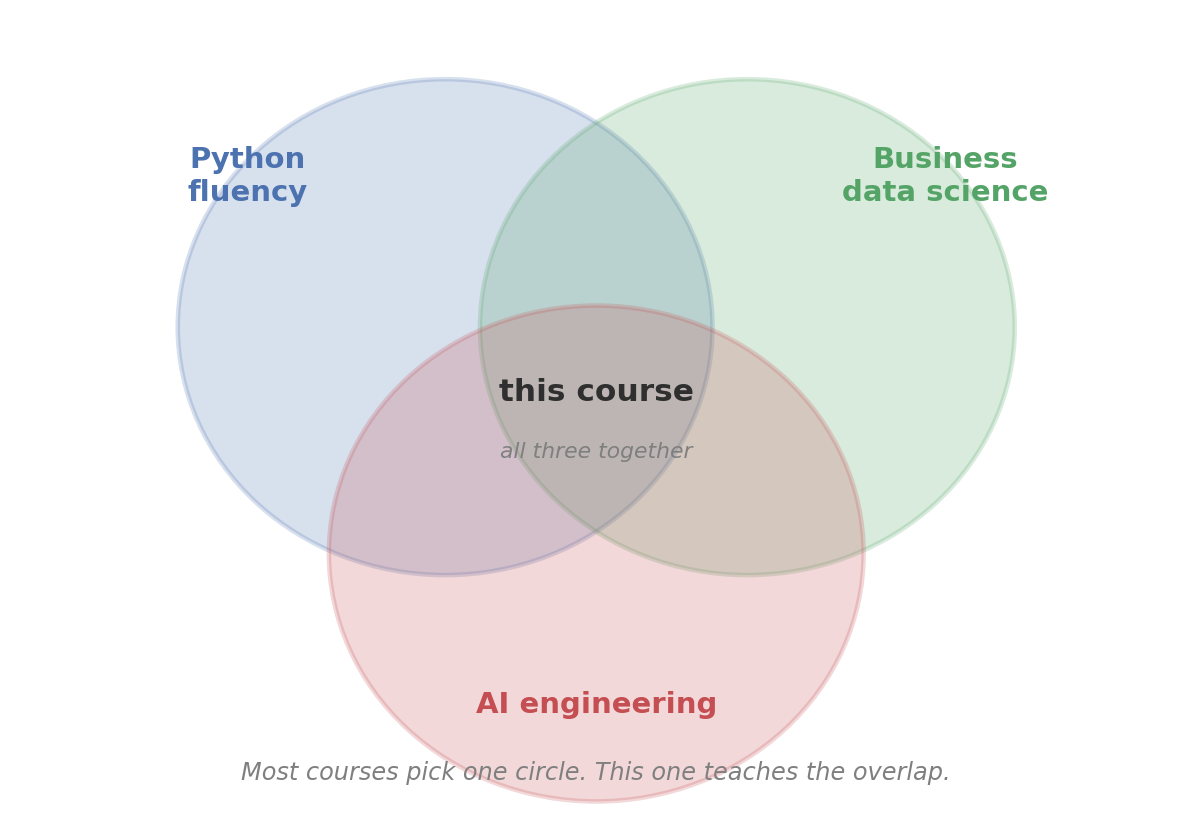
\includegraphics[width=0.9\textwidth,height=0.78\textheight,keepaspectratio]{images/06_three_circles.png}
  \end{center}
  \note{%
    \textbf{$\sim$4 min.} Point: this is not a pure programming course, not a pure statistics course, and not a prompt-engineering course --- it is the overlap.\\[2pt]
    The overlap is the employable part: plenty of people can do one circle. Doing all three is what lets you take a business problem and return a working, defensible system.\\[2pt]
    \textbf{Ask the room:} ``Which circle are you strongest in?'' Useful for you (calibrates pace) and for them (they find their pairs).
  }
\end{frame}

\begin{frame}{Three skills, taught together}
  \begin{block}{1. Python fluency}
    Read, write, and modify clean Python without friction. Functions, modules, error handling, defensive parsing.
  \end{block}
  \begin{exampleblock}{2. Working with data professionally}
    pandas, NumPy, matplotlib, scikit-learn, statistics, time-series forecasting --- plus PyTorch deep learning for when the classical toolkit stops. Real datasets, not toy ones.
  \end{exampleblock}
  \begin{block}{3. AI-driven automation}
    Calling LLMs as functions. Structured output. Retrieval-augmented generation. Tools and agents. Document processing. \emph{Plus} the engineering wrapper around all of it.
  \end{block}
  \note{%
    \textbf{$\sim$6 min.} Point: name the three skills concretely so ``AI course'' stops being vague.\\[2pt]
    \textbf{The phrase to land is ``LLMs as functions.''} Most students arrive thinking of AI as a chat window. This course treats a model as a component you call from code, with typed inputs and outputs, inside a program you control. That reframe is most of the difference between a demo and a product.\\[2pt]
    Stress ``real datasets, not toy ones'' --- they'll meet messy data early, on purpose.\\[2pt]
    ``The engineering wrapper'' is the honest bit: evaluation, cost, monitoring, deployment. It's the least glamorous and the most decisive.
  }
\end{frame}

% ============================================================
\section{Structure}
% ============================================================

\begin{frame}{Twenty modules --- 53 lessons, 7 labs (+ 14 appendices)}
  \scriptsize
  \renewcommand{\arraystretch}{0.88}%
  \begin{tabular}{rll}
    \toprule
    \textbf{\#} & \textbf{Module} & \textbf{Notebooks} \\
    \midrule
    0 & Onboarding              & master onboarding + overview + see-it-work \\
    1 & Foundations             & NB 1–6 — Python you can read without friction \\
    2 & Data science            & NB 7–11 — pandas, NumPy, plots, stats, time series \\
    3 & Real-world I/O          & NB 12–13 — HTTP, SQL, validation \\
    4 & Web scraping            & NB 14–16 — BeautifulSoup, Firecrawl, the OpenAlex API \\
    5 & Machine learning        & NB 17–19 — sklearn, model evaluation, features \\
    6 & Deep learning (PyTorch) & NB 20–22 — tensors \& the training loop, training craft, embeddings \& serving \\
    7 & Industry applications   & NB 23–26 — churn value, fraud, segmentation, demand \\
    8 & AI engineering          & NB 27–32 — LLM patterns, RAG, agents, evaluation \\
    9 & Building AI POCs        & NB 33–36 — setup, three POCs, RAG deep dive, agentic AI \\
    10 & Agents, tools \& MCP    & NB 37–40 — architectures, robust tools, MCP, multi-agent \\
    11 & NLP (optional)          & NB 41–43 — topic modeling, sentiment \\
    12 & DeepTab (optional)      & NB 44 — deep learning for tabular data \\
    13 & Production              & NB 45–46 — packaging, scheduling, config \& secrets \\
    14 & CI/CD \& deployment     & mini-book + 3 labs — Docker, GitHub Actions, HTTPS \\
    15 & Capstones               & NB 47–48 — analytics + AI assistant \\
    16 & Business AI             & NB 49–52 — strategy, architecture, BPM, governance \\
    17 & Django (optional)       & mini-book + 2 labs — serve a model behind a web UI \\
    18 & Compound AI eval (opt.) & NB 53 + lab — factorial designs, ANOVA attribution, CAFE \\
    19 & Containers (optional)   & mini-book + lab — images, layers, namespaces, Dockerfiles \\
    \bottomrule
  \end{tabular}
  \vspace{4pt}

  {\footnotesize \textbf{Every module folder has its own README} --- goals, prerequisites, what you'll build. Read it before the module's first notebook. Module and lesson numbers follow the learning order.}
  \note{%
    \textbf{$\sim$8 min.} Point: the full map. Let them \emph{scan} --- don't narrate 20 rows.\\[2pt]
    Call out only the shape: modules 1--5 are the skill spine, 7--12 the applications, 13--19 the shipping and judgement half. Then name the optional ones (11, 12, 14, 17, 18, 19) explicitly --- that's the anxiety reducer.\\[2pt]
    \textbf{The footnote is the actionable instruction:} every module has a README with goals and prerequisites. Students who skip them get lost; students who read them never wonder whether they're ready.\\[2pt]
    \textbf{Ask the room:} ``Anything here you're surprised to see in an AI course?'' Usually CI/CD or Django --- and the answer is the whole thesis: shipping is the job.\\[2pt]
    \emph{Maintainer note:} the counts on this slide and the study slide are hand-maintained. If you've added a module, re-check them against the repo README.
  }
\end{frame}

\begin{frame}{Module dependencies — what comes before what}
  \begin{center}
    
\includegraphics[width=\textwidth,height=0.82\textheight,keepaspectratio]{images/01_dependency_graph.png}
  \end{center}
  \note{%
    \textbf{$\sim$5 min.} Point: it is a graph, not a queue --- several modules are safe to take in any order once their upstreams are done.\\[2pt]
    Use it to answer the question they're all silently asking: ``can I skip ahead to the AI parts?'' Follow the edges into module 8 --- it needs 3 and 5. Skipping means you'll be debugging pandas errors instead of learning AI engineering.\\[2pt]
    Note module 19 sits as a root: it needs only Module-1 Python and a terminal, so it can be read any time --- before or after module 14.\\[2pt]
    This graph is generated from the repo's module tables, so it stays true after a renumber.
  }
\end{frame}

% ============================================================
\section{Learning paths}
% ============================================================

\begin{frame}{Pick the path that fits you}
  \begin{center}
    
\includegraphics[width=\textwidth,height=0.82\textheight,keepaspectratio]{images/02_learning_paths.png}
  \end{center}
  \note{%
    \textbf{$\sim$4 min.} Point: five paths, wildly different time budgets --- 10 h to 125 h. Nobody does all of it unless they want to.\\[2pt]
    Let them find their row and read across. The greyed dots are modules that path skips, and skipping is \emph{endorsed}, not a compromise.\\[2pt]
    For a taught cohort, say plainly which path your syllabus follows and which modules are examinable --- otherwise this slide creates uncertainty rather than removing it.\\[2pt]
    Next slide has the detail; keep this one to orientation.
  }
\end{frame}

\begin{frame}{When to pick which path}
  \begin{block}{Complete beginner}
    Never written code before. Take all modules in \textbf{spiral order} (see it work first, then the skills, then the builds). Time-budget: \textbf{about 125 hours} — the interactive estimator in \texttt{00b} computes yours.
  \end{block}
  \begin{exampleblock}{Analyst who knows Excel and SQL}
    Skim Module 1 (Python basics); Module 3's SQL will feel familiar. Focus on Modules 2 (data science), 4 (web scraping), 5 (ML), 7 (industry applications), 15 (capstone). Time-budget: \textbf{about 47 hours}.
  \end{exampleblock}
  \begin{block}{ML practitioner adding AI engineering}
    Skip foundations and data science. Focus on Modules 6 (PyTorch), 8 (AI engineering), 10 (agents \& MCP), 13 (production), 15 (capstone). Time-budget: \textbf{about 38 hours}.
  \end{block}
  \note{%
    \textbf{$\sim$8 min.} Point: give explicit permission to skip. The most common failure is a capable analyst grinding through Module 1 out of duty and quitting from boredom.\\[2pt]
    The instruction that matters: \textbf{skim, don't skip blind.} Open the module README, check the goals, and if you can already do all of them, move on --- and come back the moment something doesn't parse.\\[2pt]
    \textbf{The hour figures are honest and worth defending} --- 125 hours for a true beginner. Underselling it produces dropouts at week three. The estimator in notebook 00b computes a personal number from their answers.\\[2pt]
    \textbf{Ask the room:} ``Which of these three is closest to you?'' Hands up per path --- tells you instantly what pace the cohort needs.
  }
\end{frame}

\begin{frame}{Twelve weeks, self-paced}
  \begin{center}
    
\includegraphics[width=\textwidth,height=0.65\textheight,keepaspectratio]{images/03_weekly_timeline.png}
  \end{center}
  Got more time? Move faster. Got less? Split one week into two.
  \note{%
    \textbf{$\sim$4 min.} Point: a concrete, self-paced 12-week shape --- 8--15 h/week. This is the answer to ``how long will this actually take?''\\[2pt]
    Note the weeks are not uniform: week 11 (POCs $+$ agents) is the heaviest at $\sim$15 h. Flag it now so it isn't a surprise.\\[2pt]
    \textbf{If you're teaching this as a taught course, say clearly that this is the self-paced plan and your lecture schedule differs} --- otherwise students try to follow both. The fast track's 12-lecture plan is the taught-course version.\\[2pt]
    The line to say: consistency beats intensity. Six focused hours a week for twelve weeks beats two heroic weekends.
  }
\end{frame}

% ============================================================
\section{How to study}
% ============================================================

\begin{frame}{The five-step study loop}
  \begin{center}
    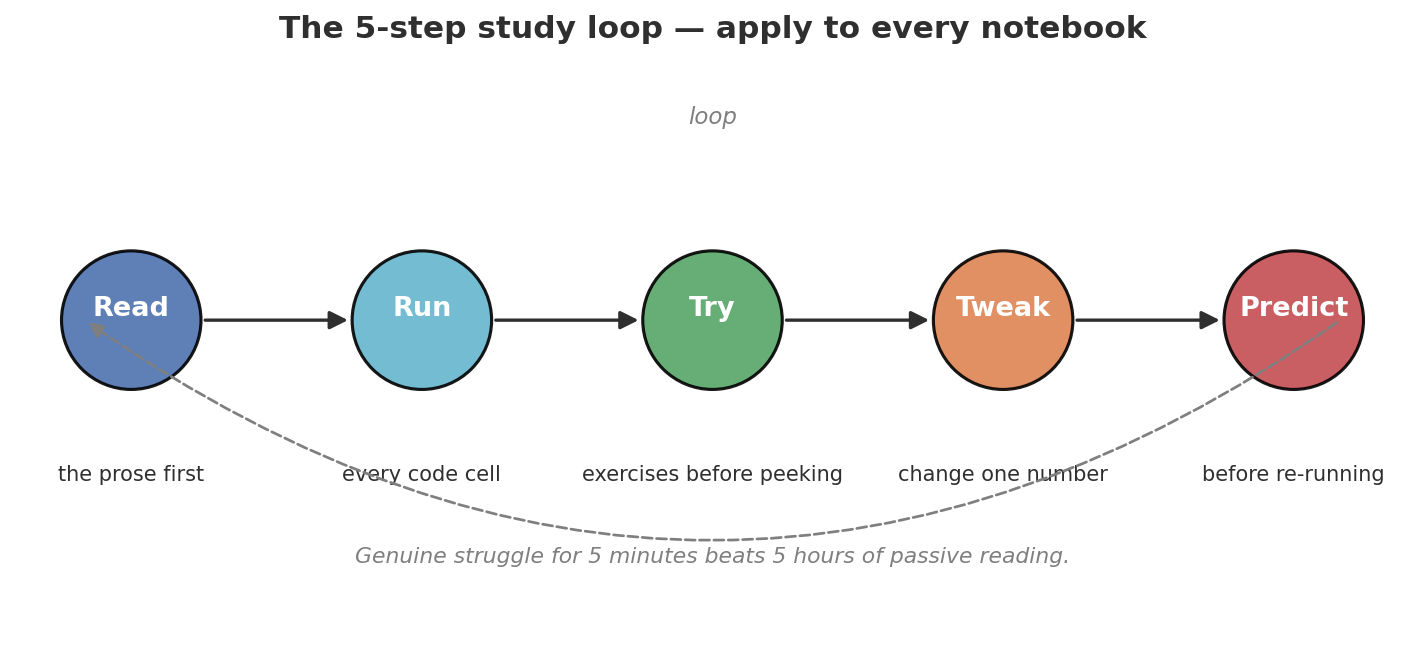
\includegraphics[width=\textwidth,height=0.65\textheight,keepaspectratio]{images/04_study_loop.png}
  \end{center}
  Apply this loop to \emph{every} notebook. Genuine struggle beats passive reading.
  \note{%
    \textbf{$\sim$6 min --- the highest-value slide for outcomes.}\\[2pt]
    Point: \emph{how} to study, not what. Read $\to$ Run $\to$ Try $\to$ Tweak $\to$ Predict.\\[2pt]
    \textbf{Predict-before-you-run is the step that does the work} and the one everyone drops. Saying the expected output out loud before pressing shift-enter converts passive reading into a test with immediate feedback. When the prediction is wrong, that's the learning moment.\\[2pt]
    Be blunt about the failure mode: running every cell and watching output scroll past feels productive and teaches almost nothing. Ask them how they'd know the difference the next morning.\\[2pt]
    \textbf{Ask the room:} ``Who has read a whole tutorial and remembered none of it?'' Every hand. That's why this slide exists.
  }
\end{frame}

\begin{frame}{Eight visual markers you'll see throughout}
  \footnotesize
  \begin{tabular}{ll}
    \toprule
    \textbf{Marker} & \textbf{Meaning} \\
    \midrule
    \texttt{(Tip)}            & A small ``stop and notice'' callout. \\
    \texttt{(Intuition)}      & The mental model behind the syntax. \\
    \texttt{(Pitfall)}        & A bug or anti-pattern that bites if you're not warned. \\
    \texttt{(Quick exercise)} & A $\sim$2-minute in-lesson checkpoint with a collapsible solution. \\
    \texttt{(Exercises)}      & Hands-on tasks. Try \emph{before} peeking at the solution. \\
    \texttt{(Bonus)}          & One larger applied task per notebook. \\
    \texttt{(Debug me)}       & A cell that \emph{intentionally} contains a bug for you to find. \\
    \texttt{(Next step)}      & Always points to the next notebook in your path. \\
    \bottomrule
  \end{tabular}
  \vspace{4pt}

  Once you internalise the markers they become road signs, not decoration.
  \note{%
    \textbf{$\sim$5 min.} Point: the notebooks have a consistent visual grammar --- learn it once, navigate 117 notebooks.\\[2pt]
    The two to dwell on: \textbf{Quick exercise} (a $\sim$2-minute checkpoint with a collapsible solution --- the rhythm of every lesson) and \textbf{Debug me} (a cell that is \emph{intentionally} broken).\\[2pt]
    \textbf{Warn them explicitly about Debug me}, or someone will spend twenty minutes assuming the course has a typo. The bug is the exercise.\\[2pt]
    Tell them to resist opening solutions early --- reading a solution feels like understanding and isn't. The struggle is where the learning is.
  }
\end{frame}

\begin{frame}{Checkpoints, quizzes, and the fast track}
  \begin{block}{322 in-lesson checkpoints --- the rhythm of every lesson}
    Roughly every $\sim$20 minutes of material: a \texttt{(Quick exercise)} with a scaffolded starter and a collapsible solution --- every solution executed in a fresh kernel. Teach $\to$ try for $\sim$2 minutes $\to$ reveal.
  \end{block}
  \begin{exampleblock}{17 module quizzes}
    Five multiple-choice questions per content module ($\sim$10 minutes) in \texttt{quizzes/} --- read code, predict behaviour, pick the right tool. Score 0--2/5? Re-do the module before moving on.
  \end{exampleblock}
  \begin{block}{Short on time? The fast track}
    \texttt{fast\_track/} condenses the whole course into 22 trimmed lessons ($\sim$26 hours) --- the 14 core essentials plus 8 breadth extensions.
  \end{block}
  \note{%
    \textbf{$\sim$6 min.} Point: three feedback mechanisms at three timescales --- checkpoints (minutes), quizzes (per module), fast track (an alternative route).\\[2pt]
    \textbf{If you're teaching live, this slide is about you as much as them:} the 322 checkpoints are the built-in pause points. Teach $\sim$20 min, set the checkpoint, give them $\sim$2 min, reveal. That's the lecture rhythm, and it needs no preparation.\\[2pt]
    The quiz rule is worth stating plainly: score 0--2 out of 5 and redo the module before moving on. The dependency graph means weak foundations compound.\\[2pt]
    Mention the fast track exists but don't oversell it to a taught cohort --- it's for people with a hard time budget, and it trims depth to get there.
  }
\end{frame}

% ============================================================
\section{What you'll build}
% ============================================================

\begin{frame}{Six small artefacts you ship along the way}
  \begin{center}
    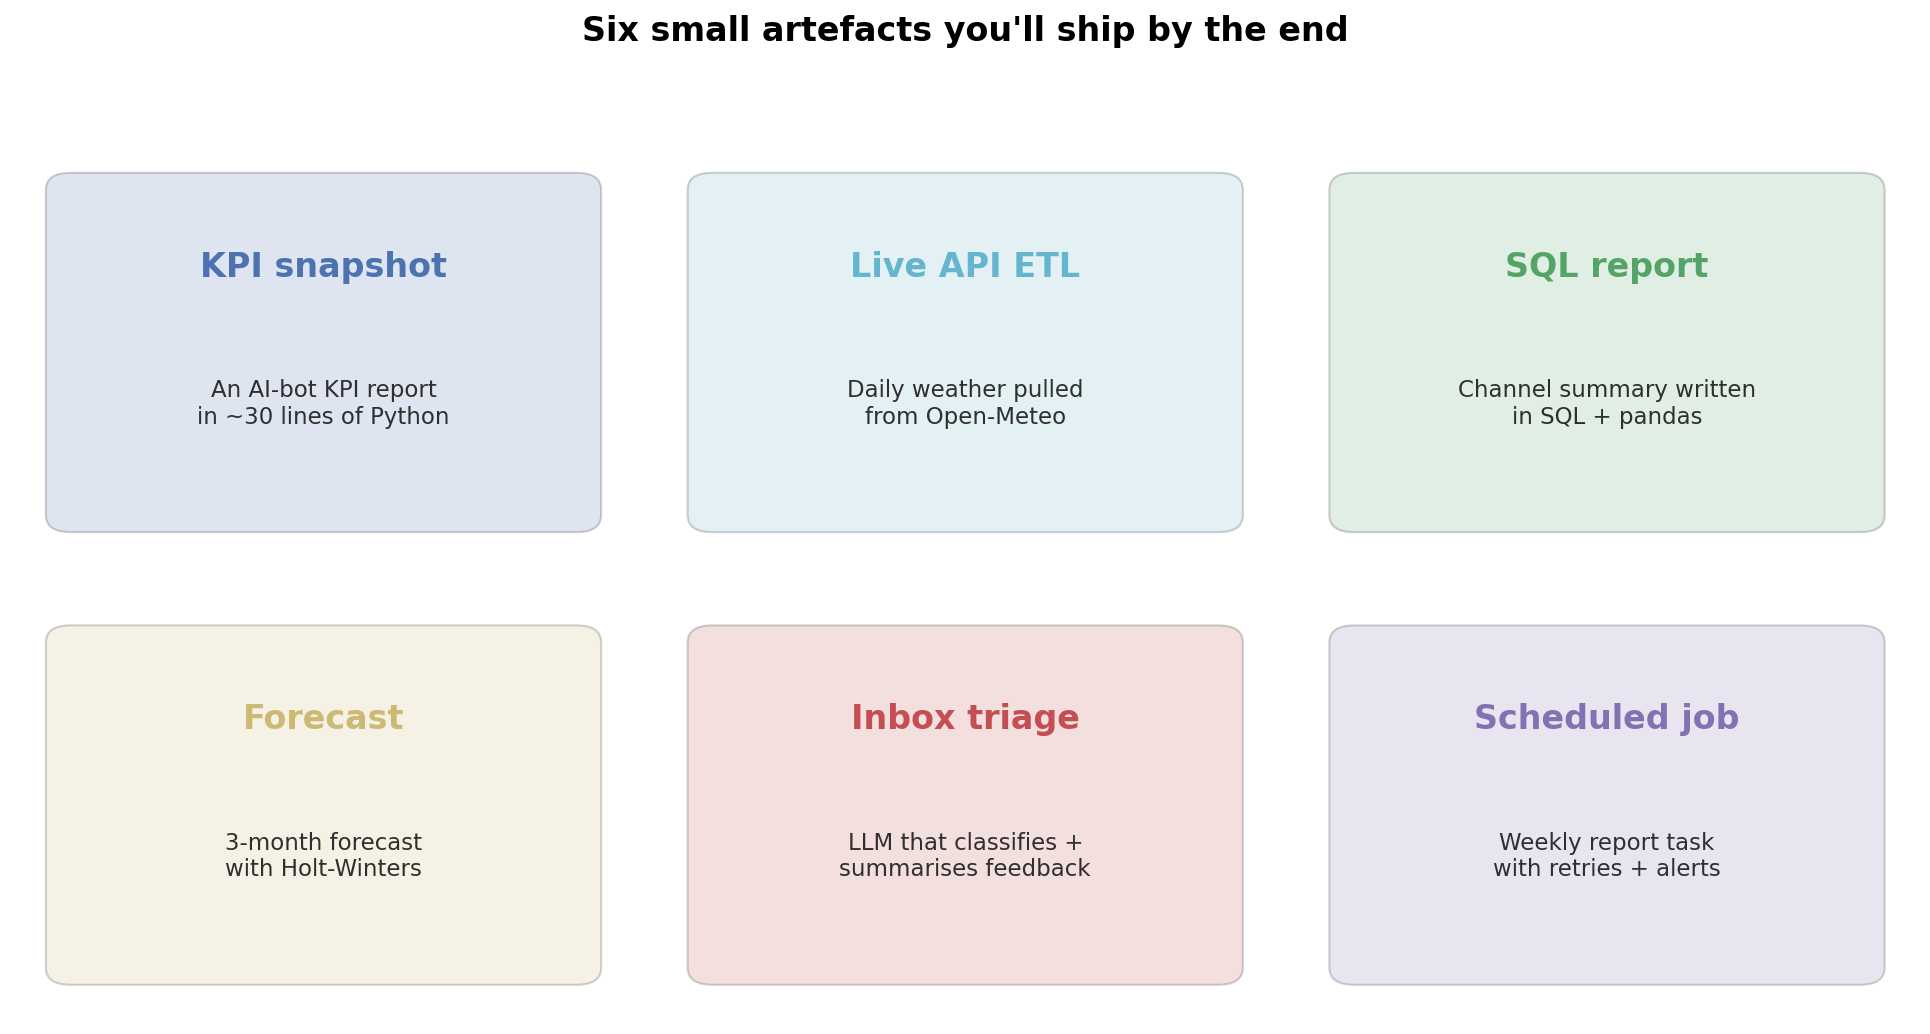
\includegraphics[width=\textwidth,height=0.82\textheight,keepaspectratio]{images/05_what_youll_build.png}
  \end{center}
  \note{%
    \textbf{$\sim$5 min.} Point: they finish with things that exist, not just notes. Motivation slide --- keep the energy up.\\[2pt]
    The framing that lands with career-minded students: these are portfolio pieces you can show and \emph{explain}. Being able to defend a design decision in an interview is what separates them from someone who followed a tutorial.\\[2pt]
    Keep it brief --- the detail is in the modules, and the capstones are on the next slide.
  }
\end{frame}

\begin{frame}{Plus two big capstones at the end}
  \begin{exampleblock}{Capstone A — AI Support-Bot Analytics (NB 47)}
    Five channels × twelve months of operational data $\to$ 2$\times$2 executive dashboard $\to$ regression demonstrating Simpson's paradox $\to$ five-bullet executive summary.
  \end{exampleblock}
  \vspace{6pt}
  \begin{block}{Capstone B — AI Customer-Feedback Assistant (NB 48)}
    Ingest free-form customer feedback $\to$ classify + extract via the MockLLM $\to$ ground answers in a knowledge base via RAG $\to$ orchestrate as a scheduled job with alerts. End-to-end AI feature.
  \end{block}
  \note{%
    \textbf{$\sim$6 min.} Point: two capstones, deliberately different --- A is the analytics story, B is the AI system.\\[2pt]
    \textbf{Capstone A's real lesson is Simpson's paradox} --- the aggregate trend reverses when you segment. It's the single most useful statistical trap for anyone presenting numbers to management, and it lands far harder in a project than on a slide.\\[2pt]
    Capstone B is the whole AI-engineering stack in one artefact: classify, extract, ground with RAG, schedule, alert. If they can explain that pipeline, they can hold a technical conversation about production AI.\\[2pt]
    Both end in a \emph{decision or a summary a manager could act on} --- that's the course's signature, and it's what makes them portfolio-worthy.
  }
\end{frame}

% ============================================================
\section{Getting started}
% ============================================================

\begin{frame}{LLM providers — local and hosted, four options}
  \footnotesize
  \begin{tabular}{lll}
    \toprule
    \textbf{Provider} & \textbf{Class} & \textbf{Best for} \\
    \midrule
    OpenAI    & \texttt{OpenAILLM("gpt-5.4-mini")}            & Reliable default \\
    Anthropic & \texttt{AnthropicLLM("claude-haiku-4-5")}    & Long context, careful tone \\
    Google    & \texttt{GoogleLLM("gemini-2.5-flash")}       & Cheapest at high volume \\
    Ollama    & \texttt{OllamaLLM("llama3.2:3b")}            & \textbf{Local} -- no internet, no key \\
    \bottomrule
  \end{tabular}
  \vspace{6pt}
  \begin{block}{Default = the offline MockLLM}
    Every AI notebook runs offline by default. Swapping in a real provider is a
    \emph{one-line} change thanks to the unified interface in
    \texttt{llm\_providers.py} at the repo root.
  \end{block}
  \vspace{4pt}
  \begin{exampleblock}{See the dedicated guide}
    Notebook \texttt{08\_ai\_engineering/A1\_llm\_providers\_guide.ipynb} has the
    full setup walk-through, model recommendations, and cost estimates.
  \end{exampleblock}
  \note{%
    \textbf{$\sim$6 min.} Point: the course is \textbf{100\,\% offline by default}. Say this early and clearly --- it removes the biggest barrier and the biggest anxiety.\\[2pt]
    \textbf{Nobody needs an API key, a credit card, or an account to complete this course.} Every AI notebook runs against a built-in MockLLM. Repeat it; students who half-heard it will worry for weeks.\\[2pt]
    Swapping in a real provider is a one-line change through the shared interface in \texttt{llm\_providers.py} --- that's a service-oriented boundary, and NB 50 names it as one.\\[2pt]
    \emph{Maintainer note:} the model names here mirror the defaults in \texttt{llm\_providers.py}. If you update one, update the other --- and expect this table to date quickly.
  }
\end{frame}


\begin{frame}[fragile]{What you need to install}
  \begin{block}{For Google Colab}
    Nothing. All required libraries are pre-installed. Open the notebook, hit Shift+Enter.
  \end{block}
  \begin{exampleblock}{For local Jupyter}
\small
\begin{verbatim}
python -m venv .venv
source .venv/bin/activate
pip install -r requirements.txt
jupyter lab
\end{verbatim}
  \end{exampleblock}
  Notebook 0 includes an environment-check cell you run to confirm everything works before you move on.
  \note{%
    \textbf{$\sim$8 min --- and budget more if this is session one with a fresh cohort.}\\[2pt]
    Point: two routes in. \textbf{Colab needs nothing} --- that is the answer for anyone whose laptop is fighting them, and it takes setup off the critical path entirely.\\[2pt]
    \textbf{If you're teaching live, do the local setup with the room now}, not later. Environment problems are the number-one reason people quietly stop, and they're much cheaper to fix with a neighbour than alone at home. Expect the usual: wrong Python version, activation not persisting, corporate proxies.\\[2pt]
    Point everyone at the environment-check cell in notebook 0 --- it's the definitive answer to ``is my setup right?''\\[2pt]
    \textbf{Have the Colab link ready as the escape hatch} for anyone still stuck after ten minutes; move on and debug in the break.
  }
\end{frame}

\begin{frame}[fragile]{Now → open Notebook 0}
  \vspace{8pt}
  \begin{center}
    {\large One file to open. The rest unfolds from there.}\\[14pt]
    \texttt{\large 00\_onboarding/00\_master\_onboarding.ipynb}\\[18pt]
  \end{center}
  \begin{block}{Three things that notebook does for you}
    \begin{enumerate}
      \item Confirms your Python environment is correctly set up.
      \item Explains the five-step study loop you'll use throughout.
      \item Helps you pick the right learning path from the five options.
    \end{enumerate}
  \end{block}
  \note{%
    \textbf{$\sim$4 min.} Point: reduce the whole deck to one action --- open one file.\\[2pt]
    The most common way to fail at this course is never starting because 117 notebooks feels like too much. One file. The rest unfolds.\\[2pt]
    \textbf{If you have five minutes, open it on screen now} and let them watch the environment check run. Seeing it work is worth more than describing it.\\[2pt]
    If your cohort is following a fixed syllabus, say so here so nobody spends an evening on the path-picker.
  }
\end{frame}

\begin{frame}{One last reminder before you start}
  \begin{block}{Five-step study loop, in your pocket}
    \textbf{Read} the prose first $\to$ \textbf{Run} every code cell $\to$
    \textbf{Try} the exercises before peeking $\to$ \textbf{Tweak} one number $\to$
    \textbf{Predict} the new output before re-running.
  \end{block}
  \begin{exampleblock}{When to use which marker}
    \texttt{(Tip)} information; \texttt{(Intuition)} mental model;
    \texttt{(Pitfall)} avoid this; \texttt{(Quick exercise)} $\sim$2-minute checkpoint;
    \texttt{(Exercise)} hands-on practice; \texttt{(Bonus)} bigger applied task;
    \texttt{(Debug me)} intentional bug — find it.
  \end{exampleblock}
  \begin{alertblock}{When you're stuck for 15 minutes}
    Copy the full error into a search engine. 95\% of beginner errors are
    well-documented. The course is designed to teach you to debug, not to
    spare you the experience.
  \end{alertblock}
  \note{%
    \textbf{$\sim$5 min.} Point: the debugging attitude. This is the slide that keeps people from quitting in week two.\\[2pt]
    \textbf{Normalise the errors:} a red traceback is not a sign they're unsuited to this. Professionals see them all day; the difference is they read them instead of panicking. Tell them to read the \emph{last} line first.\\[2pt]
    The 15-minute rule is a real technique --- struggle is productive up to a point, then it's just attrition. Search the exact error text, then ask a person.\\[2pt]
    Nice callback: NB 27 explains \emph{why} the assistant will confidently invent a fix; NB 51 gives the review checklist. The course teaches supervision, not avoidance.\\[2pt]
    If you're teaching live, this is where you name your office hours or forum. Say it concretely.
  }
\end{frame}

\begin{frame}
  \begin{center}
    {\Huge\bfseries Welcome.}\\[10pt]
    \large 117 notebooks await you.\\[20pt]
    {\large \textit{Open Module 0 next.}}
  \end{center}
  \note{%
    \textbf{$\sim$2 min --- close warmly and stop.}\\[2pt]
    Point: end on the invitation, not on logistics. Resist adding one more announcement here.\\[2pt]
    If you want one closing line, make it the promise the course actually keeps: \emph{by the end, you will have shipped something that runs, and you'll be able to explain every part of it.}\\[2pt]
    Then give the single next action out loud --- open \texttt{00\_master\_onboarding.ipynb} before the next session --- and take questions.
  }
\end{frame}

\end{document}
"
\ifdefined\notesmode
  \usepackage{pgfpages}
  \setbeameroption{show notes on second screen=right}
\fi

% Theme
\usetheme{Madrid}
\usecolortheme{default}
\setbeamertemplate{navigation symbols}{}
\setbeamertemplate{footline}[frame number]
\setbeamertemplate{blocks}[rounded][shadow=false]
\setbeamertemplate{headline}{%
  \leavevmode%
  \hbox{%
    \begin{beamercolorbox}[wd=\paperwidth,ht=2.5ex,dp=1.125ex]{section in head/foot}%
      \insertsectionnavigationhorizontal{\paperwidth}{}{\hskip0pt plus1filll}%
    \end{beamercolorbox}%
  }%
}
\AtBeginSection[]{%
  \begin{frame}{Outline}
    \tableofcontents[currentsection,sectionstyle=show/shaded,subsectionstyle=show/show/hide]
  \end{frame}
}

\title{Course Overview}
\subtitle{Python for AI-Driven Automation and Business Data Science}
\author{Course materials}
\institute{}
\date{}

\begin{document}

\begin{frame}\titlepage\end{frame}

\begin{frame}{Contents}
  \tableofcontents[hideallsubsections]
\end{frame}

% ============================================================
\section{The big picture}
% ============================================================

\begin{frame}{The course in one diagram}
  \begin{center}
    
\includegraphics[width=\textwidth,height=0.78\textheight,keepaspectratio]{images/00_course_roadmap.png}
  \end{center}
  \note{%
    \textbf{$\sim$5 min.} Point: show the whole shape once, so everything later has somewhere to attach.\\[2pt]
    Trace the spine with a finger --- Python $\to$ data $\to$ ML $\to$ AI $\to$ shipping --- and say the one sentence that matters: \textbf{each module is a prerequisite for the next, so the order is not arbitrary.}\\[2pt]
    Point out the starred optional modules now to defuse the intimidation: 20 modules is not 20 obligations.\\[2pt]
    \textbf{Do not read the boxes aloud.} They will read faster than you can speak, and the detail comes three slides later.
  }
\end{frame}

\begin{frame}{Where this course sits}
  \begin{center}
    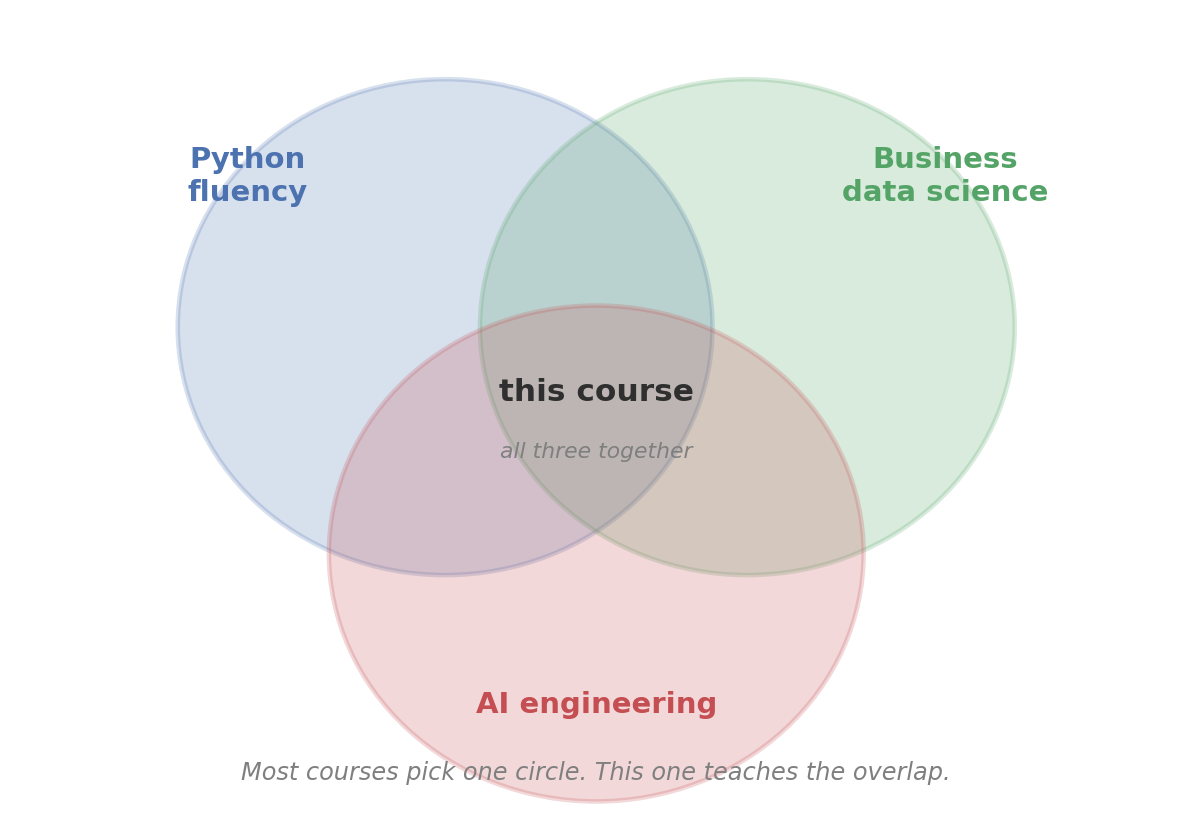
\includegraphics[width=0.9\textwidth,height=0.78\textheight,keepaspectratio]{images/06_three_circles.png}
  \end{center}
  \note{%
    \textbf{$\sim$4 min.} Point: this is not a pure programming course, not a pure statistics course, and not a prompt-engineering course --- it is the overlap.\\[2pt]
    The overlap is the employable part: plenty of people can do one circle. Doing all three is what lets you take a business problem and return a working, defensible system.\\[2pt]
    \textbf{Ask the room:} ``Which circle are you strongest in?'' Useful for you (calibrates pace) and for them (they find their pairs).
  }
\end{frame}

\begin{frame}{Three skills, taught together}
  \begin{block}{1. Python fluency}
    Read, write, and modify clean Python without friction. Functions, modules, error handling, defensive parsing.
  \end{block}
  \begin{exampleblock}{2. Working with data professionally}
    pandas, NumPy, matplotlib, scikit-learn, statistics, time-series forecasting --- plus PyTorch deep learning for when the classical toolkit stops. Real datasets, not toy ones.
  \end{exampleblock}
  \begin{block}{3. AI-driven automation}
    Calling LLMs as functions. Structured output. Retrieval-augmented generation. Tools and agents. Document processing. \emph{Plus} the engineering wrapper around all of it.
  \end{block}
  \note{%
    \textbf{$\sim$6 min.} Point: name the three skills concretely so ``AI course'' stops being vague.\\[2pt]
    \textbf{The phrase to land is ``LLMs as functions.''} Most students arrive thinking of AI as a chat window. This course treats a model as a component you call from code, with typed inputs and outputs, inside a program you control. That reframe is most of the difference between a demo and a product.\\[2pt]
    Stress ``real datasets, not toy ones'' --- they'll meet messy data early, on purpose.\\[2pt]
    ``The engineering wrapper'' is the honest bit: evaluation, cost, monitoring, deployment. It's the least glamorous and the most decisive.
  }
\end{frame}

% ============================================================
\section{Structure}
% ============================================================

\begin{frame}{Twenty modules --- 53 lessons, 7 labs (+ 14 appendices)}
  \scriptsize
  \renewcommand{\arraystretch}{0.88}%
  \begin{tabular}{rll}
    \toprule
    \textbf{\#} & \textbf{Module} & \textbf{Notebooks} \\
    \midrule
    0 & Onboarding              & master onboarding + overview + see-it-work \\
    1 & Foundations             & NB 1–6 — Python you can read without friction \\
    2 & Data science            & NB 7–11 — pandas, NumPy, plots, stats, time series \\
    3 & Real-world I/O          & NB 12–13 — HTTP, SQL, validation \\
    4 & Web scraping            & NB 14–16 — BeautifulSoup, Firecrawl, the OpenAlex API \\
    5 & Machine learning        & NB 17–19 — sklearn, model evaluation, features \\
    6 & Deep learning (PyTorch) & NB 20–22 — tensors \& the training loop, training craft, embeddings \& serving \\
    7 & Industry applications   & NB 23–26 — churn value, fraud, segmentation, demand \\
    8 & AI engineering          & NB 27–32 — LLM patterns, RAG, agents, evaluation \\
    9 & Building AI POCs        & NB 33–36 — setup, three POCs, RAG deep dive, agentic AI \\
    10 & Agents, tools \& MCP    & NB 37–40 — architectures, robust tools, MCP, multi-agent \\
    11 & NLP (optional)          & NB 41–43 — topic modeling, sentiment \\
    12 & DeepTab (optional)      & NB 44 — deep learning for tabular data \\
    13 & Production              & NB 45–46 — packaging, scheduling, config \& secrets \\
    14 & CI/CD \& deployment     & mini-book + 3 labs — Docker, GitHub Actions, HTTPS \\
    15 & Capstones               & NB 47–48 — analytics + AI assistant \\
    16 & Business AI             & NB 49–52 — strategy, architecture, BPM, governance \\
    17 & Django (optional)       & mini-book + 2 labs — serve a model behind a web UI \\
    18 & Compound AI eval (opt.) & NB 53 + lab — factorial designs, ANOVA attribution, CAFE \\
    19 & Containers (optional)   & mini-book + lab — images, layers, namespaces, Dockerfiles \\
    \bottomrule
  \end{tabular}
  \vspace{4pt}

  {\footnotesize \textbf{Every module folder has its own README} --- goals, prerequisites, what you'll build. Read it before the module's first notebook. Module and lesson numbers follow the learning order.}
  \note{%
    \textbf{$\sim$8 min.} Point: the full map. Let them \emph{scan} --- don't narrate 20 rows.\\[2pt]
    Call out only the shape: modules 1--5 are the skill spine, 7--12 the applications, 13--19 the shipping and judgement half. Then name the optional ones (11, 12, 14, 17, 18, 19) explicitly --- that's the anxiety reducer.\\[2pt]
    \textbf{The footnote is the actionable instruction:} every module has a README with goals and prerequisites. Students who skip them get lost; students who read them never wonder whether they're ready.\\[2pt]
    \textbf{Ask the room:} ``Anything here you're surprised to see in an AI course?'' Usually CI/CD or Django --- and the answer is the whole thesis: shipping is the job.\\[2pt]
    \emph{Maintainer note:} the counts on this slide and the study slide are hand-maintained. If you've added a module, re-check them against the repo README.
  }
\end{frame}

\begin{frame}{Module dependencies — what comes before what}
  \begin{center}
    
\includegraphics[width=\textwidth,height=0.82\textheight,keepaspectratio]{images/01_dependency_graph.png}
  \end{center}
  \note{%
    \textbf{$\sim$5 min.} Point: it is a graph, not a queue --- several modules are safe to take in any order once their upstreams are done.\\[2pt]
    Use it to answer the question they're all silently asking: ``can I skip ahead to the AI parts?'' Follow the edges into module 8 --- it needs 3 and 5. Skipping means you'll be debugging pandas errors instead of learning AI engineering.\\[2pt]
    Note module 19 sits as a root: it needs only Module-1 Python and a terminal, so it can be read any time --- before or after module 14.\\[2pt]
    This graph is generated from the repo's module tables, so it stays true after a renumber.
  }
\end{frame}

% ============================================================
\section{Learning paths}
% ============================================================

\begin{frame}{Pick the path that fits you}
  \begin{center}
    
\includegraphics[width=\textwidth,height=0.82\textheight,keepaspectratio]{images/02_learning_paths.png}
  \end{center}
  \note{%
    \textbf{$\sim$4 min.} Point: five paths, wildly different time budgets --- 10 h to 125 h. Nobody does all of it unless they want to.\\[2pt]
    Let them find their row and read across. The greyed dots are modules that path skips, and skipping is \emph{endorsed}, not a compromise.\\[2pt]
    For a taught cohort, say plainly which path your syllabus follows and which modules are examinable --- otherwise this slide creates uncertainty rather than removing it.\\[2pt]
    Next slide has the detail; keep this one to orientation.
  }
\end{frame}

\begin{frame}{When to pick which path}
  \begin{block}{Complete beginner}
    Never written code before. Take all modules in \textbf{spiral order} (see it work first, then the skills, then the builds). Time-budget: \textbf{about 125 hours} — the interactive estimator in \texttt{00b} computes yours.
  \end{block}
  \begin{exampleblock}{Analyst who knows Excel and SQL}
    Skim Module 1 (Python basics); Module 3's SQL will feel familiar. Focus on Modules 2 (data science), 4 (web scraping), 5 (ML), 7 (industry applications), 15 (capstone). Time-budget: \textbf{about 47 hours}.
  \end{exampleblock}
  \begin{block}{ML practitioner adding AI engineering}
    Skip foundations and data science. Focus on Modules 6 (PyTorch), 8 (AI engineering), 10 (agents \& MCP), 13 (production), 15 (capstone). Time-budget: \textbf{about 38 hours}.
  \end{block}
  \note{%
    \textbf{$\sim$8 min.} Point: give explicit permission to skip. The most common failure is a capable analyst grinding through Module 1 out of duty and quitting from boredom.\\[2pt]
    The instruction that matters: \textbf{skim, don't skip blind.} Open the module README, check the goals, and if you can already do all of them, move on --- and come back the moment something doesn't parse.\\[2pt]
    \textbf{The hour figures are honest and worth defending} --- 125 hours for a true beginner. Underselling it produces dropouts at week three. The estimator in notebook 00b computes a personal number from their answers.\\[2pt]
    \textbf{Ask the room:} ``Which of these three is closest to you?'' Hands up per path --- tells you instantly what pace the cohort needs.
  }
\end{frame}

\begin{frame}{Twelve weeks, self-paced}
  \begin{center}
    
\includegraphics[width=\textwidth,height=0.65\textheight,keepaspectratio]{images/03_weekly_timeline.png}
  \end{center}
  Got more time? Move faster. Got less? Split one week into two.
  \note{%
    \textbf{$\sim$4 min.} Point: a concrete, self-paced 12-week shape --- 8--15 h/week. This is the answer to ``how long will this actually take?''\\[2pt]
    Note the weeks are not uniform: week 11 (POCs $+$ agents) is the heaviest at $\sim$15 h. Flag it now so it isn't a surprise.\\[2pt]
    \textbf{If you're teaching this as a taught course, say clearly that this is the self-paced plan and your lecture schedule differs} --- otherwise students try to follow both. The fast track's 12-lecture plan is the taught-course version.\\[2pt]
    The line to say: consistency beats intensity. Six focused hours a week for twelve weeks beats two heroic weekends.
  }
\end{frame}

% ============================================================
\section{How to study}
% ============================================================

\begin{frame}{The five-step study loop}
  \begin{center}
    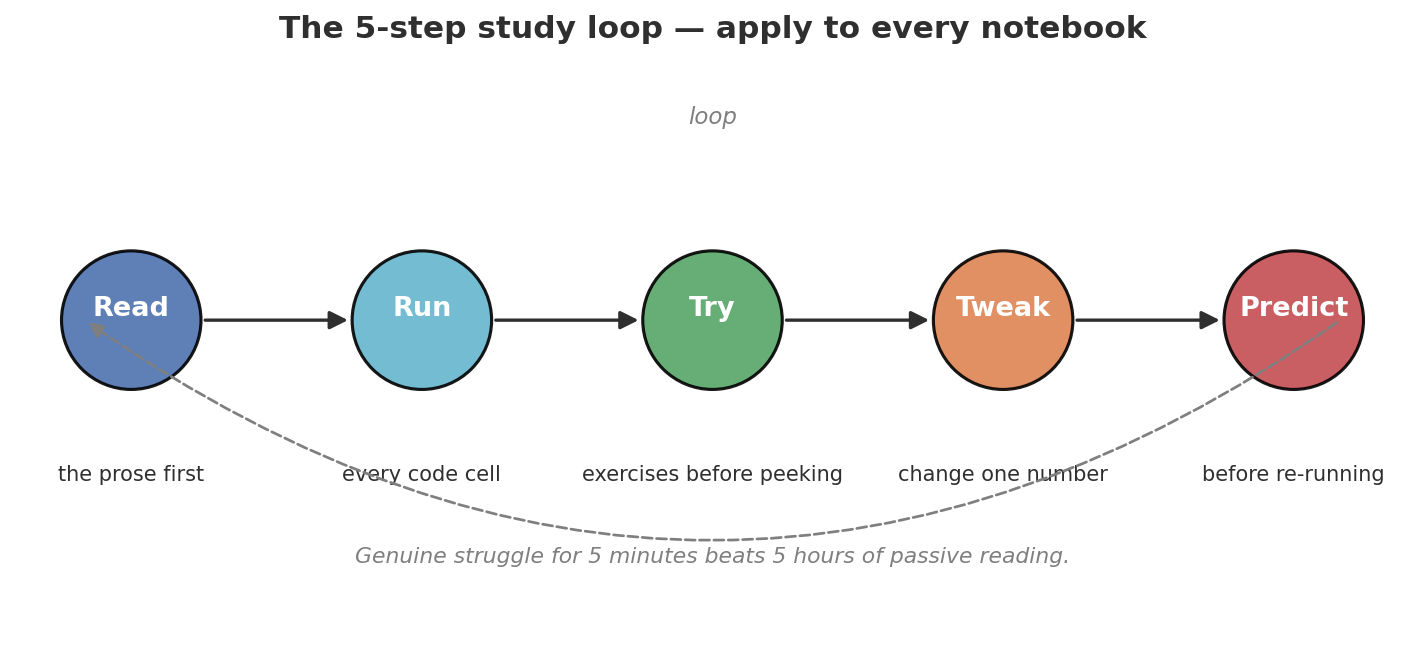
\includegraphics[width=\textwidth,height=0.65\textheight,keepaspectratio]{images/04_study_loop.png}
  \end{center}
  Apply this loop to \emph{every} notebook. Genuine struggle beats passive reading.
  \note{%
    \textbf{$\sim$6 min --- the highest-value slide for outcomes.}\\[2pt]
    Point: \emph{how} to study, not what. Read $\to$ Run $\to$ Try $\to$ Tweak $\to$ Predict.\\[2pt]
    \textbf{Predict-before-you-run is the step that does the work} and the one everyone drops. Saying the expected output out loud before pressing shift-enter converts passive reading into a test with immediate feedback. When the prediction is wrong, that's the learning moment.\\[2pt]
    Be blunt about the failure mode: running every cell and watching output scroll past feels productive and teaches almost nothing. Ask them how they'd know the difference the next morning.\\[2pt]
    \textbf{Ask the room:} ``Who has read a whole tutorial and remembered none of it?'' Every hand. That's why this slide exists.
  }
\end{frame}

\begin{frame}{Eight visual markers you'll see throughout}
  \footnotesize
  \begin{tabular}{ll}
    \toprule
    \textbf{Marker} & \textbf{Meaning} \\
    \midrule
    \texttt{(Tip)}            & A small ``stop and notice'' callout. \\
    \texttt{(Intuition)}      & The mental model behind the syntax. \\
    \texttt{(Pitfall)}        & A bug or anti-pattern that bites if you're not warned. \\
    \texttt{(Quick exercise)} & A $\sim$2-minute in-lesson checkpoint with a collapsible solution. \\
    \texttt{(Exercises)}      & Hands-on tasks. Try \emph{before} peeking at the solution. \\
    \texttt{(Bonus)}          & One larger applied task per notebook. \\
    \texttt{(Debug me)}       & A cell that \emph{intentionally} contains a bug for you to find. \\
    \texttt{(Next step)}      & Always points to the next notebook in your path. \\
    \bottomrule
  \end{tabular}
  \vspace{4pt}

  Once you internalise the markers they become road signs, not decoration.
  \note{%
    \textbf{$\sim$5 min.} Point: the notebooks have a consistent visual grammar --- learn it once, navigate 117 notebooks.\\[2pt]
    The two to dwell on: \textbf{Quick exercise} (a $\sim$2-minute checkpoint with a collapsible solution --- the rhythm of every lesson) and \textbf{Debug me} (a cell that is \emph{intentionally} broken).\\[2pt]
    \textbf{Warn them explicitly about Debug me}, or someone will spend twenty minutes assuming the course has a typo. The bug is the exercise.\\[2pt]
    Tell them to resist opening solutions early --- reading a solution feels like understanding and isn't. The struggle is where the learning is.
  }
\end{frame}

\begin{frame}{Checkpoints, quizzes, and the fast track}
  \begin{block}{322 in-lesson checkpoints --- the rhythm of every lesson}
    Roughly every $\sim$20 minutes of material: a \texttt{(Quick exercise)} with a scaffolded starter and a collapsible solution --- every solution executed in a fresh kernel. Teach $\to$ try for $\sim$2 minutes $\to$ reveal.
  \end{block}
  \begin{exampleblock}{17 module quizzes}
    Five multiple-choice questions per content module ($\sim$10 minutes) in \texttt{quizzes/} --- read code, predict behaviour, pick the right tool. Score 0--2/5? Re-do the module before moving on.
  \end{exampleblock}
  \begin{block}{Short on time? The fast track}
    \texttt{fast\_track/} condenses the whole course into 22 trimmed lessons ($\sim$26 hours) --- the 14 core essentials plus 8 breadth extensions.
  \end{block}
  \note{%
    \textbf{$\sim$6 min.} Point: three feedback mechanisms at three timescales --- checkpoints (minutes), quizzes (per module), fast track (an alternative route).\\[2pt]
    \textbf{If you're teaching live, this slide is about you as much as them:} the 322 checkpoints are the built-in pause points. Teach $\sim$20 min, set the checkpoint, give them $\sim$2 min, reveal. That's the lecture rhythm, and it needs no preparation.\\[2pt]
    The quiz rule is worth stating plainly: score 0--2 out of 5 and redo the module before moving on. The dependency graph means weak foundations compound.\\[2pt]
    Mention the fast track exists but don't oversell it to a taught cohort --- it's for people with a hard time budget, and it trims depth to get there.
  }
\end{frame}

% ============================================================
\section{What you'll build}
% ============================================================

\begin{frame}{Six small artefacts you ship along the way}
  \begin{center}
    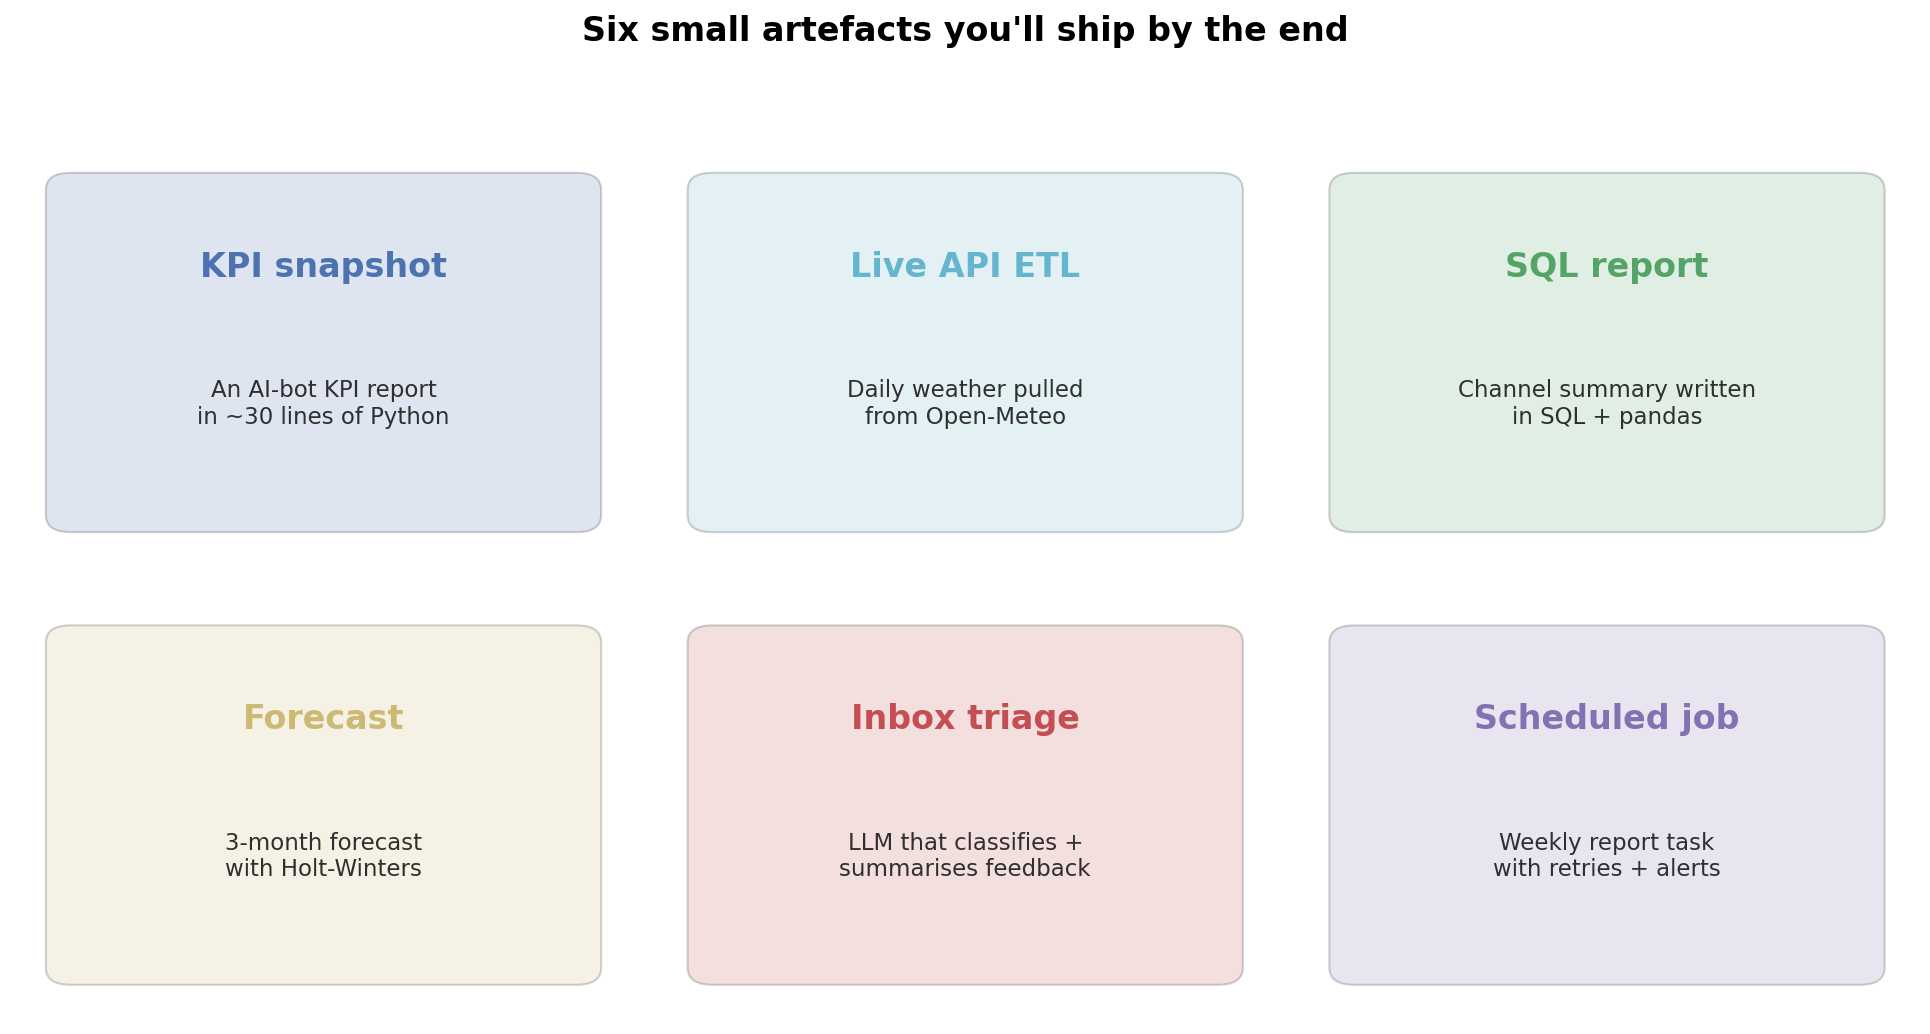
\includegraphics[width=\textwidth,height=0.82\textheight,keepaspectratio]{images/05_what_youll_build.png}
  \end{center}
  \note{%
    \textbf{$\sim$5 min.} Point: they finish with things that exist, not just notes. Motivation slide --- keep the energy up.\\[2pt]
    The framing that lands with career-minded students: these are portfolio pieces you can show and \emph{explain}. Being able to defend a design decision in an interview is what separates them from someone who followed a tutorial.\\[2pt]
    Keep it brief --- the detail is in the modules, and the capstones are on the next slide.
  }
\end{frame}

\begin{frame}{Plus two big capstones at the end}
  \begin{exampleblock}{Capstone A — AI Support-Bot Analytics (NB 47)}
    Five channels × twelve months of operational data $\to$ 2$\times$2 executive dashboard $\to$ regression demonstrating Simpson's paradox $\to$ five-bullet executive summary.
  \end{exampleblock}
  \vspace{6pt}
  \begin{block}{Capstone B — AI Customer-Feedback Assistant (NB 48)}
    Ingest free-form customer feedback $\to$ classify + extract via the MockLLM $\to$ ground answers in a knowledge base via RAG $\to$ orchestrate as a scheduled job with alerts. End-to-end AI feature.
  \end{block}
  \note{%
    \textbf{$\sim$6 min.} Point: two capstones, deliberately different --- A is the analytics story, B is the AI system.\\[2pt]
    \textbf{Capstone A's real lesson is Simpson's paradox} --- the aggregate trend reverses when you segment. It's the single most useful statistical trap for anyone presenting numbers to management, and it lands far harder in a project than on a slide.\\[2pt]
    Capstone B is the whole AI-engineering stack in one artefact: classify, extract, ground with RAG, schedule, alert. If they can explain that pipeline, they can hold a technical conversation about production AI.\\[2pt]
    Both end in a \emph{decision or a summary a manager could act on} --- that's the course's signature, and it's what makes them portfolio-worthy.
  }
\end{frame}

% ============================================================
\section{Getting started}
% ============================================================

\begin{frame}{LLM providers — local and hosted, four options}
  \footnotesize
  \begin{tabular}{lll}
    \toprule
    \textbf{Provider} & \textbf{Class} & \textbf{Best for} \\
    \midrule
    OpenAI    & \texttt{OpenAILLM("gpt-5.4-mini")}            & Reliable default \\
    Anthropic & \texttt{AnthropicLLM("claude-haiku-4-5")}    & Long context, careful tone \\
    Google    & \texttt{GoogleLLM("gemini-2.5-flash")}       & Cheapest at high volume \\
    Ollama    & \texttt{OllamaLLM("llama3.2:3b")}            & \textbf{Local} -- no internet, no key \\
    \bottomrule
  \end{tabular}
  \vspace{6pt}
  \begin{block}{Default = the offline MockLLM}
    Every AI notebook runs offline by default. Swapping in a real provider is a
    \emph{one-line} change thanks to the unified interface in
    \texttt{llm\_providers.py} at the repo root.
  \end{block}
  \vspace{4pt}
  \begin{exampleblock}{See the dedicated guide}
    Notebook \texttt{08\_ai\_engineering/A1\_llm\_providers\_guide.ipynb} has the
    full setup walk-through, model recommendations, and cost estimates.
  \end{exampleblock}
  \note{%
    \textbf{$\sim$6 min.} Point: the course is \textbf{100\,\% offline by default}. Say this early and clearly --- it removes the biggest barrier and the biggest anxiety.\\[2pt]
    \textbf{Nobody needs an API key, a credit card, or an account to complete this course.} Every AI notebook runs against a built-in MockLLM. Repeat it; students who half-heard it will worry for weeks.\\[2pt]
    Swapping in a real provider is a one-line change through the shared interface in \texttt{llm\_providers.py} --- that's a service-oriented boundary, and NB 50 names it as one.\\[2pt]
    \emph{Maintainer note:} the model names here mirror the defaults in \texttt{llm\_providers.py}. If you update one, update the other --- and expect this table to date quickly.
  }
\end{frame}


\begin{frame}[fragile]{What you need to install}
  \begin{block}{For Google Colab}
    Nothing. All required libraries are pre-installed. Open the notebook, hit Shift+Enter.
  \end{block}
  \begin{exampleblock}{For local Jupyter}
\small
\begin{verbatim}
python -m venv .venv
source .venv/bin/activate
pip install -r requirements.txt
jupyter lab
\end{verbatim}
  \end{exampleblock}
  Notebook 0 includes an environment-check cell you run to confirm everything works before you move on.
  \note{%
    \textbf{$\sim$8 min --- and budget more if this is session one with a fresh cohort.}\\[2pt]
    Point: two routes in. \textbf{Colab needs nothing} --- that is the answer for anyone whose laptop is fighting them, and it takes setup off the critical path entirely.\\[2pt]
    \textbf{If you're teaching live, do the local setup with the room now}, not later. Environment problems are the number-one reason people quietly stop, and they're much cheaper to fix with a neighbour than alone at home. Expect the usual: wrong Python version, activation not persisting, corporate proxies.\\[2pt]
    Point everyone at the environment-check cell in notebook 0 --- it's the definitive answer to ``is my setup right?''\\[2pt]
    \textbf{Have the Colab link ready as the escape hatch} for anyone still stuck after ten minutes; move on and debug in the break.
  }
\end{frame}

\begin{frame}[fragile]{Now → open Notebook 0}
  \vspace{8pt}
  \begin{center}
    {\large One file to open. The rest unfolds from there.}\\[14pt]
    \texttt{\large 00\_onboarding/00\_master\_onboarding.ipynb}\\[18pt]
  \end{center}
  \begin{block}{Three things that notebook does for you}
    \begin{enumerate}
      \item Confirms your Python environment is correctly set up.
      \item Explains the five-step study loop you'll use throughout.
      \item Helps you pick the right learning path from the five options.
    \end{enumerate}
  \end{block}
  \note{%
    \textbf{$\sim$4 min.} Point: reduce the whole deck to one action --- open one file.\\[2pt]
    The most common way to fail at this course is never starting because 117 notebooks feels like too much. One file. The rest unfolds.\\[2pt]
    \textbf{If you have five minutes, open it on screen now} and let them watch the environment check run. Seeing it work is worth more than describing it.\\[2pt]
    If your cohort is following a fixed syllabus, say so here so nobody spends an evening on the path-picker.
  }
\end{frame}

\begin{frame}{One last reminder before you start}
  \begin{block}{Five-step study loop, in your pocket}
    \textbf{Read} the prose first $\to$ \textbf{Run} every code cell $\to$
    \textbf{Try} the exercises before peeking $\to$ \textbf{Tweak} one number $\to$
    \textbf{Predict} the new output before re-running.
  \end{block}
  \begin{exampleblock}{When to use which marker}
    \texttt{(Tip)} information; \texttt{(Intuition)} mental model;
    \texttt{(Pitfall)} avoid this; \texttt{(Quick exercise)} $\sim$2-minute checkpoint;
    \texttt{(Exercise)} hands-on practice; \texttt{(Bonus)} bigger applied task;
    \texttt{(Debug me)} intentional bug — find it.
  \end{exampleblock}
  \begin{alertblock}{When you're stuck for 15 minutes}
    Copy the full error into a search engine. 95\% of beginner errors are
    well-documented. The course is designed to teach you to debug, not to
    spare you the experience.
  \end{alertblock}
  \note{%
    \textbf{$\sim$5 min.} Point: the debugging attitude. This is the slide that keeps people from quitting in week two.\\[2pt]
    \textbf{Normalise the errors:} a red traceback is not a sign they're unsuited to this. Professionals see them all day; the difference is they read them instead of panicking. Tell them to read the \emph{last} line first.\\[2pt]
    The 15-minute rule is a real technique --- struggle is productive up to a point, then it's just attrition. Search the exact error text, then ask a person.\\[2pt]
    Nice callback: NB 27 explains \emph{why} the assistant will confidently invent a fix; NB 51 gives the review checklist. The course teaches supervision, not avoidance.\\[2pt]
    If you're teaching live, this is where you name your office hours or forum. Say it concretely.
  }
\end{frame}

\begin{frame}
  \begin{center}
    {\Huge\bfseries Welcome.}\\[10pt]
    \large 117 notebooks await you.\\[20pt]
    {\large \textit{Open Module 0 next.}}
  \end{center}
  \note{%
    \textbf{$\sim$2 min --- close warmly and stop.}\\[2pt]
    Point: end on the invitation, not on logistics. Resist adding one more announcement here.\\[2pt]
    If you want one closing line, make it the promise the course actually keeps: \emph{by the end, you will have shipped something that runs, and you'll be able to explain every part of it.}\\[2pt]
    Then give the single next action out loud --- open \texttt{00\_master\_onboarding.ipynb} before the next session --- and take questions.
  }
\end{frame}

\end{document}
